该实验部分采用 \(Q\)-learning 算法对多开关匹配任务进行训练。

\(Q\)-learning 是一种经典的基于值函数的强化学习算法,属于 \textbf{无模型(model-free)}、\textbf{离策略(off-policy)} 学习方法。其核心思想是通过迭代更新状态-动作值函数 \(Q(s, a)\),来逼近最优策略对应的期望累积回报。

\(Q\)-Learning 的优化目标是估计任意状态-动作对的最大可能累积回报,其策略可以通过以下贪婪方式间接得到:
\[
\pi(s) = \arg\max_a Q(s, a)
\]

在每一轮交互中,代理从当前状态 \(s_t\) 选择动作 \(a_t\),获得奖励 \(r_{t+1}\),并转移至下一个状态 \(s_{t+1}\)。\(Q\)-learning 的更新公式为:
\begin{equation}\label{eq:q-learning-update}
    Q(s_t, a_t) \leftarrow Q(s_t, a_t) + \alpha \left[ r_{t+1} + \gamma \max_{a^\prime} Q(s_{t+1}, a^\prime) - Q(s_t, a_t) \right]
\end{equation}

其中:
\begin{itemize}
    \item \(\alpha\):学习率,控制新旧信息的融合程度;
    \item \(\gamma\):折扣因子,权衡短期与长期奖励;
    \item \(\max_{a^\prime} Q(s_{t+1}, a^\prime)\):表示在下一状态下采取最优动作所能获得的最大回报。
\end{itemize}

为了兼顾探索与利用,算法常使用 \(\epsilon\)-贪婪策略(\(\epsilon\)-greedy policy),即:
\begin{itemize}
    \item 以概率 \(1 - \epsilon\) 选择当前 \(Q\) 值最大的动作(利用);
    \item 以概率 \(\epsilon\) 随机选择任一动作(探索)。
\end{itemize}

与策略梯度方法相比,\(Q\)-learning 不需要建模策略函数 \(\pi_\theta(a \mid s)\),而是直接学习最优状态-动作值函数 \(Q^*(s, a)\)。该算法在离散动作空间中表现优异,收敛性良好,但在高维或连续动作空间中往往面临维数灾难,难以扩展。

训练算法主流程与调参策略详见算法~\ref{agl:Qlearning_algorithm}。

\begin{algorithm}[htbp]
\caption{\(Q\)-Learning 算法(含 \(\epsilon\)-greedy 策略)}\label{agl:Qlearning_algorithm}
\KwIn{学习率 \(\alpha\),折扣因子 \(\gamma\),初始探索率 \(\epsilon_{\text{start}}\),最小探索率 \(\epsilon_{\text{end}}\),探索率衰减系数 \(\lambda\),训练轮数 \(E\),最大步数 \(T\)}
\KwOut{状态-动作值函数 \(Q(s,a)\)}

初始化 \(Q\) 表为全零矩阵: \(Q(s,a) = \mathbf{0}_{\left|s\right|\times\left|a\right|}\)\;

设置 \(\epsilon \leftarrow \epsilon_{\text{start}}\)\;

\For{\(\text{episode} = 1\) \KwTo \(E\)}{

    初始化环境状态 \(s_0\),置 \(t \leftarrow 0\),总奖励 \(R \leftarrow 0\)\;

    \While{状态 \(s_t\) 非终止且 \(t < T\)}{

        生成随机数 \(p \sim \mathcal{U}(0,1)\)\;

        \eIf{\(p < \epsilon\)}{
            从动作集合 \(\mathcal{A}\) 中随机选择动作 \(a_t\)\;
        }{
            贪婪选择动作:
            \[
            a_t \leftarrow \arg\max_{a \in \mathcal{A}} Q(s_t, a)
            \]
        }

        执行动作 \(a_t\),观察奖励 \(r_t\) 与下一个状态 \(s_{t+1}\)\;

        计算下一个状态最大动作值:
        \[
        Q_{\max} \leftarrow \max_{a' \in \mathcal{A}} Q(s_{t+1}, a')
        \]

        更新 \(Q\) 值:
        \[
        Q(s_t, a_t) \leftarrow Q(s_t, a_t) + \alpha \left[ r_t + \gamma Q_{\max} - Q(s_t, a_t) \right]
        \]

        累加奖励: \(R \leftarrow R + r_t\),更新状态:\(s_t \leftarrow s_{t+1}\),\(t \leftarrow t + 1\)\;
    }

    衰减探索率:
    \[
    \epsilon \leftarrow \max(\epsilon_{\text{end}}, \epsilon \cdot \lambda)
    \]

    \textbf{记录}:本轮总奖励、步数、成功与否、当前 \(\epsilon\)、当前 \(Q\) 值均值与最大值\;
}
\Return{\(Q(s,a)\)}
\end{algorithm}

\subsection{算法实现细节}

本节详细介绍 \(Q\)-learning 在 \textsf{MultiSwitchEnv} 环境中的实现细节。完整代码实现参见附录~\ref{sec:q-learning}。

\subsubsection{状态与动作表示}

本实验中,环境包含 \(3\) 个二值开关,因此状态空间为 \(2^3 = 8\) 种组合,动作空间亦为 \(2^3 = 8\) 个动作组合。为便于在表格型结构中索引,我们使用多维数组构建六维 \(Q\) 表:

\[
Q \in \mathbb{R}^{2 \times 2 \times 2 \times 2 \times 2 \times 2}
\]

前 \(3\) 维为状态维度,后 \(3\) 维为动作维度,每个状态-动作对均有唯一索引。索引由 \textsf{tuple(obs)} 与 \textsf{tuple(action)} 拼接实现。

\subsubsection{动作选择策略}

我们采用 \(\epsilon\)-greedy 策略以平衡探索与利用。每步生成随机数 \(p \sim \mathcal{U}(0,1)\),动作选择逻辑如下:

\begin{itemize}
    \item 若 \(p < \epsilon\),则从动作空间中随机采样 \(a_t \sim \texttt{action\_space.sample()}\)
    \item 否则选择最大动作值对应的动作:
    \[
    a_t \leftarrow \arg\max_{a \in \mathcal{A}} Q(s_t, a)
    \]
\end{itemize}

为便于索引最大值动作,我们使用 \textsf{np.unravel\_index(np.argmax(q\_table[obs\_idx]), shape)} 还原出原始动作维度。

\subsubsection{Q表更新与学习率控制}

在环境执行完动作 \(a_t\) 后,获取奖励 \(r_t\) 和下一个状态 \(s_{t+1}\),我们通过公式 (\ref{eq:q-learning-update}) 更新 \(Q\) 表。

每一轮训练结束后,按如下方式衰减探索率:

\[
\epsilon \leftarrow \max(\epsilon_{\text{end}}, \epsilon \cdot \lambda)
\]

\subsubsection{结果记录}

图~\ref{fig:q-learning_training_results} 展示了使用 \(Q\)-learning 算法在 MultiSwitchEnv 环境中训练 \(1000\) 轮后的六项核心指标,综合反映了训练收敛性、策略质量与探索策略动态变化。

\begin{figure}[htbp] 
    \centering 
    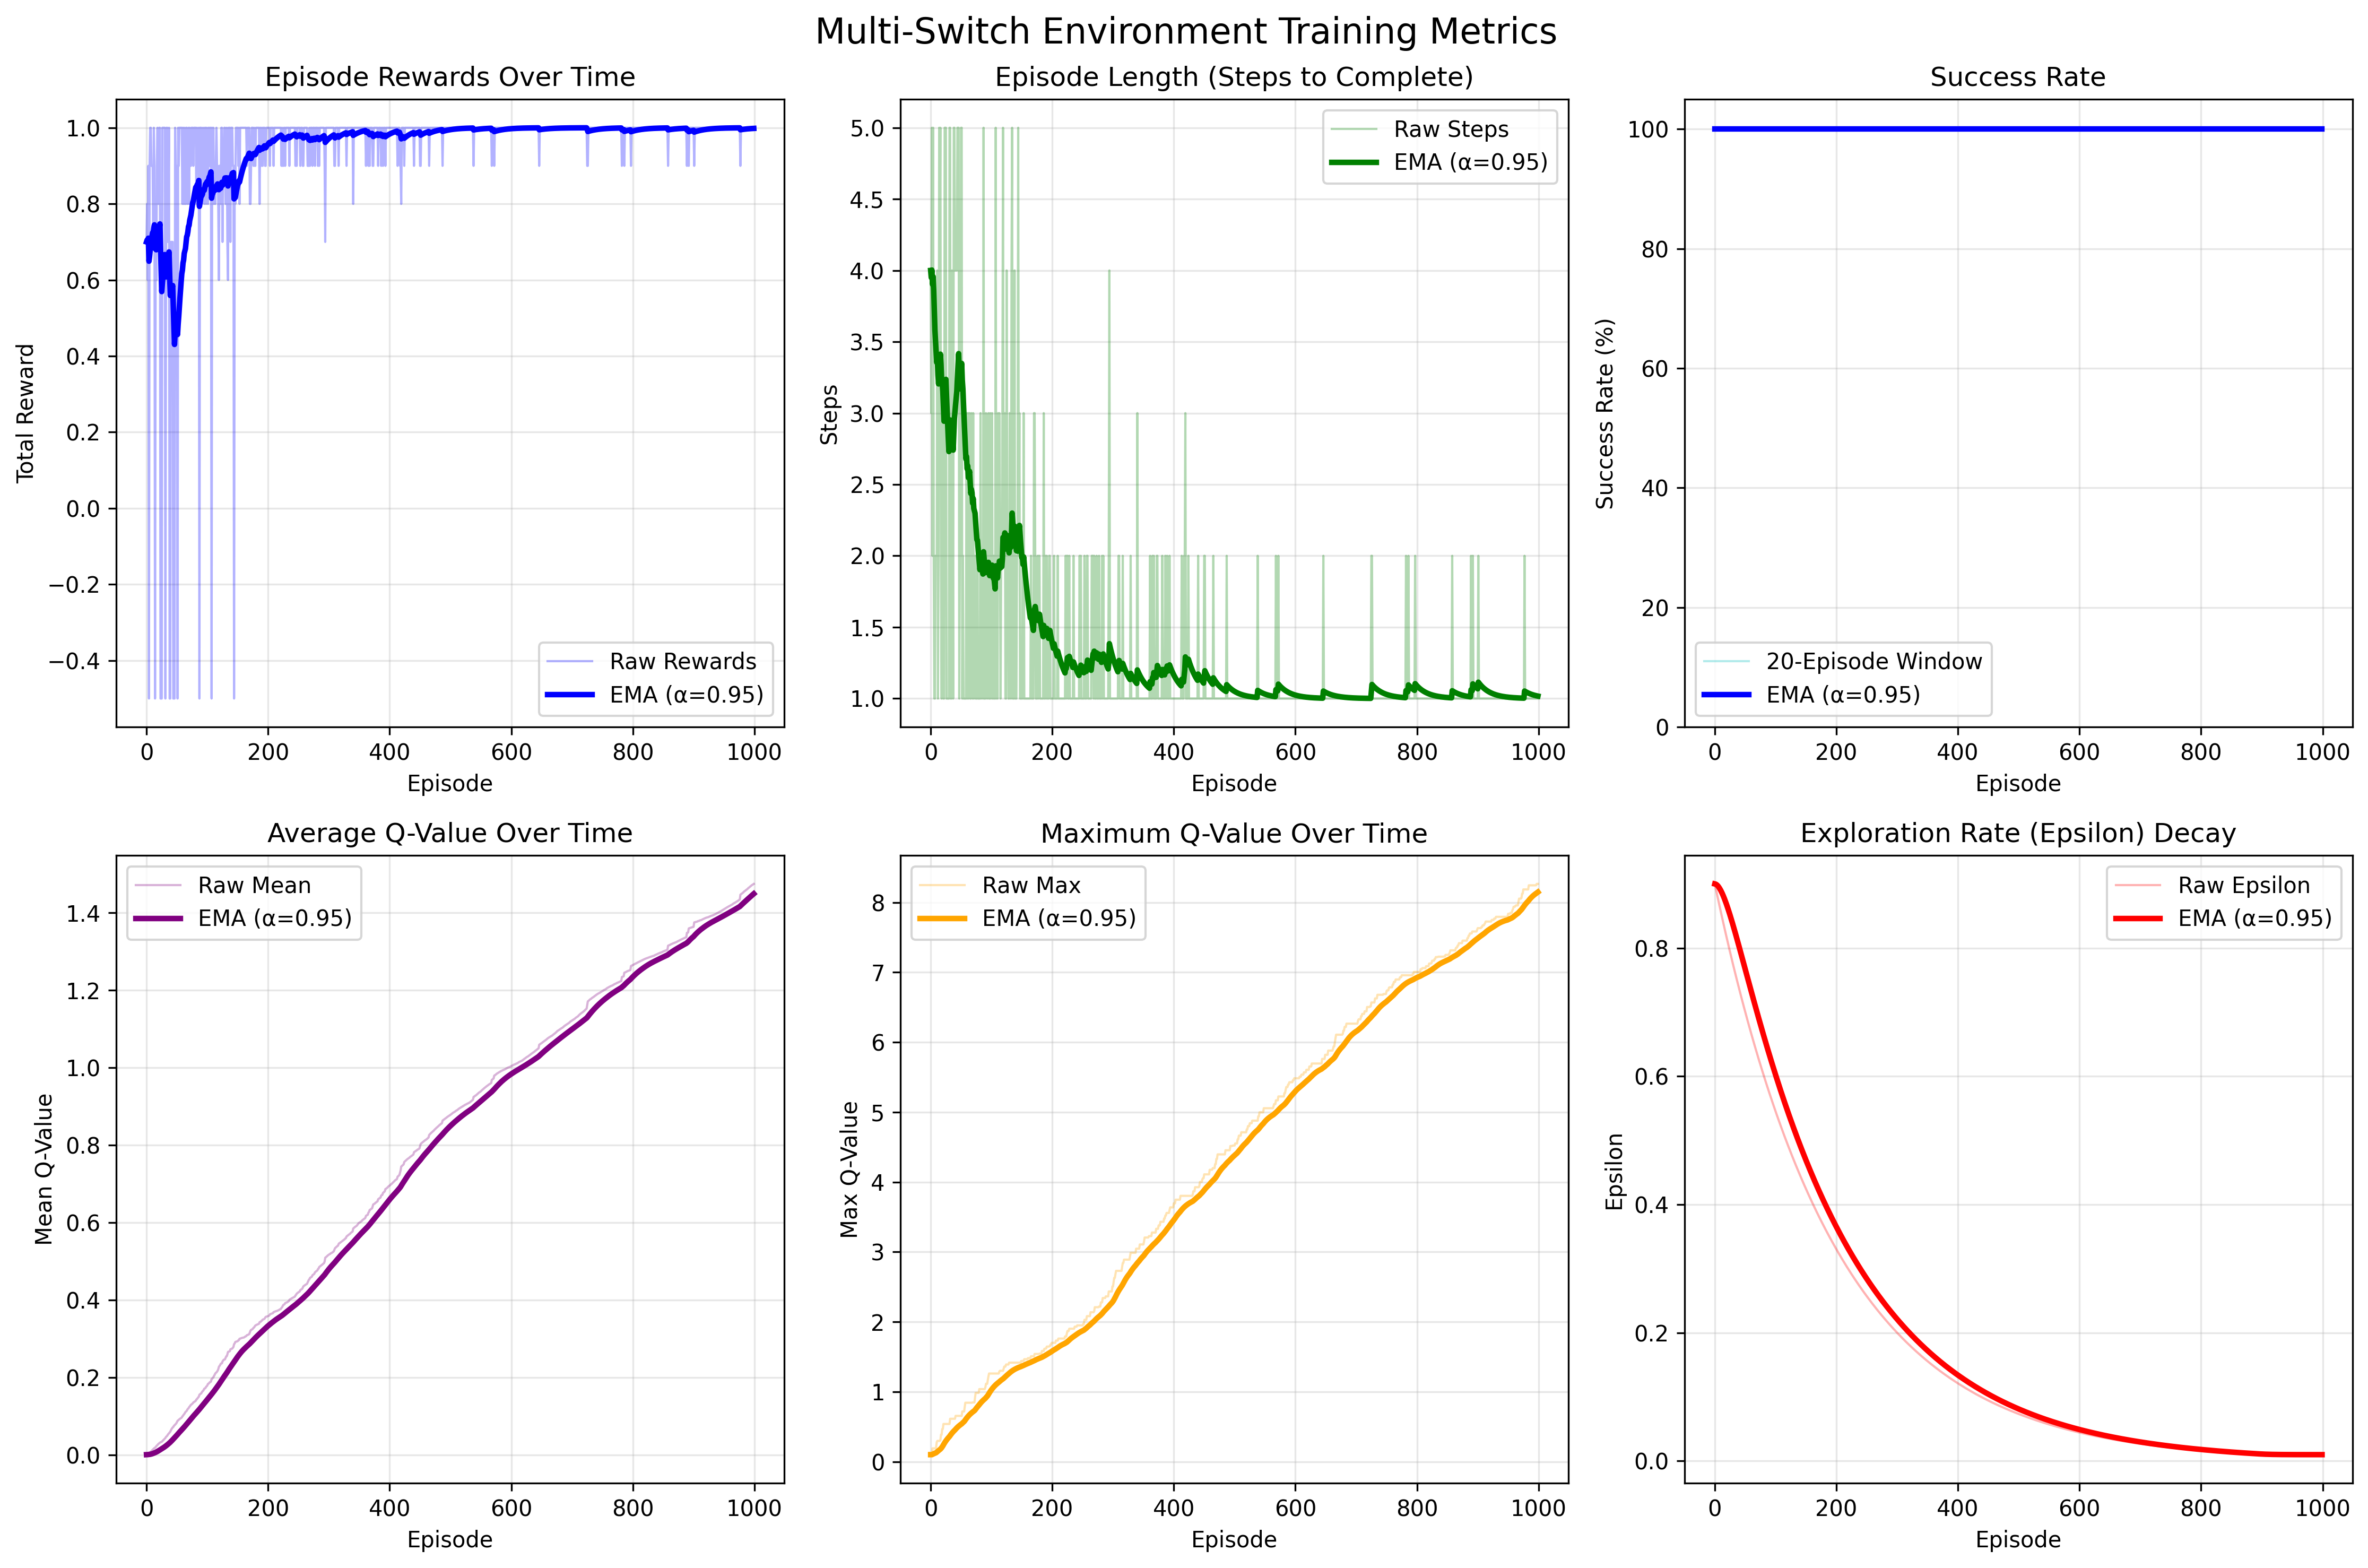
\includegraphics[width=0.9\textwidth]{figure/multi_switch/multiswitch_training_results.png} 
    \caption{\(Q\)-learning 训练过程图}\label{fig:q-learning_training_results}
\end{figure}

\begin{itemize}
    \item \textbf{每轮的奖励曲线(Episode Rewards Over Time)}:奖励曲线在前 \(200\) 轮波动较大,表明智能体仍处于试探性探索阶段;随后稳定上升至 \(1.0\),说明其成功完成任务的概率持续上升,策略趋于稳定。EMA 平滑曲线也验证了训练稳定性逐步增强。
    \item \textbf{完成任务的最大步数(Episode Length (Steps to Complete))}:步数从初始波动的 \(4\sim5\) 步迅速下降至 \(1\sim2\) 步,并最终在 \(1.0\) 附近收敛,说明智能体能够快速学习并选择高效的最优动作路径完成任务。
    \item \textbf{成功率(Success Rate)}:成功率在约 \(150\) 轮后快速提升至 \(100\%\),并维持在饱和值,显示训练已完成,策略在所有测试轮次中均成功达成任务目标。
    \item \textbf{平均 \(Q\) 值(Average Q-Value Over Time)}:平均 \(Q\) 值持续稳步上升,反映了值函数学习的累积优化过程。尤其在训练后期,其线性增长趋势表明策略学习稳定且可靠。
    \item \textbf{最大 \(Q\) 值Maximum Q-Value Over Time)}:最大 \(Q\) 值亦呈现类似趋势,从初始 \(0\) 缓慢增长至约 \(8.0\),代表智能体对某些状态-动作对的回报认知显著增强,成功识别了长期收益最优策略。
    \item \textbf{探索率衰减曲线(Exploration Rate (Epsilon) Decay)}:探索率 \(\epsilon\) 从初始的 \(0.9\) 持续衰减至 \(0.01\),符合设定的指数衰减规律。前期高探索促进了策略多样性与充分训练,后期低探索则保证了收敛策略的确定性与执行稳定性。
\end{itemize}

从整体来看,\(Q\)-learning 算法在本任务中表现出色,收敛速度快、策略稳定、\(Q\) 值函数收敛良好,成功率接近达成 \(100\%\),验证了该方法在离散状态-动作空间环境中的高效性和可靠性。

同时,我们也绘制了 \(Q\) 表随着时间演化的快照,如图~\ref{fig:qvalue_snapshots} 所示,从 Episode \(100\) 到 \(1000\),可观察到 \(Q\) 值在空间分布上逐步收敛,表明策略逐渐趋于稳定并识别出高回报状态-动作对。

\begin{figure}[htbp]
    \centering

    \begin{minipage}{0.45\textwidth}
        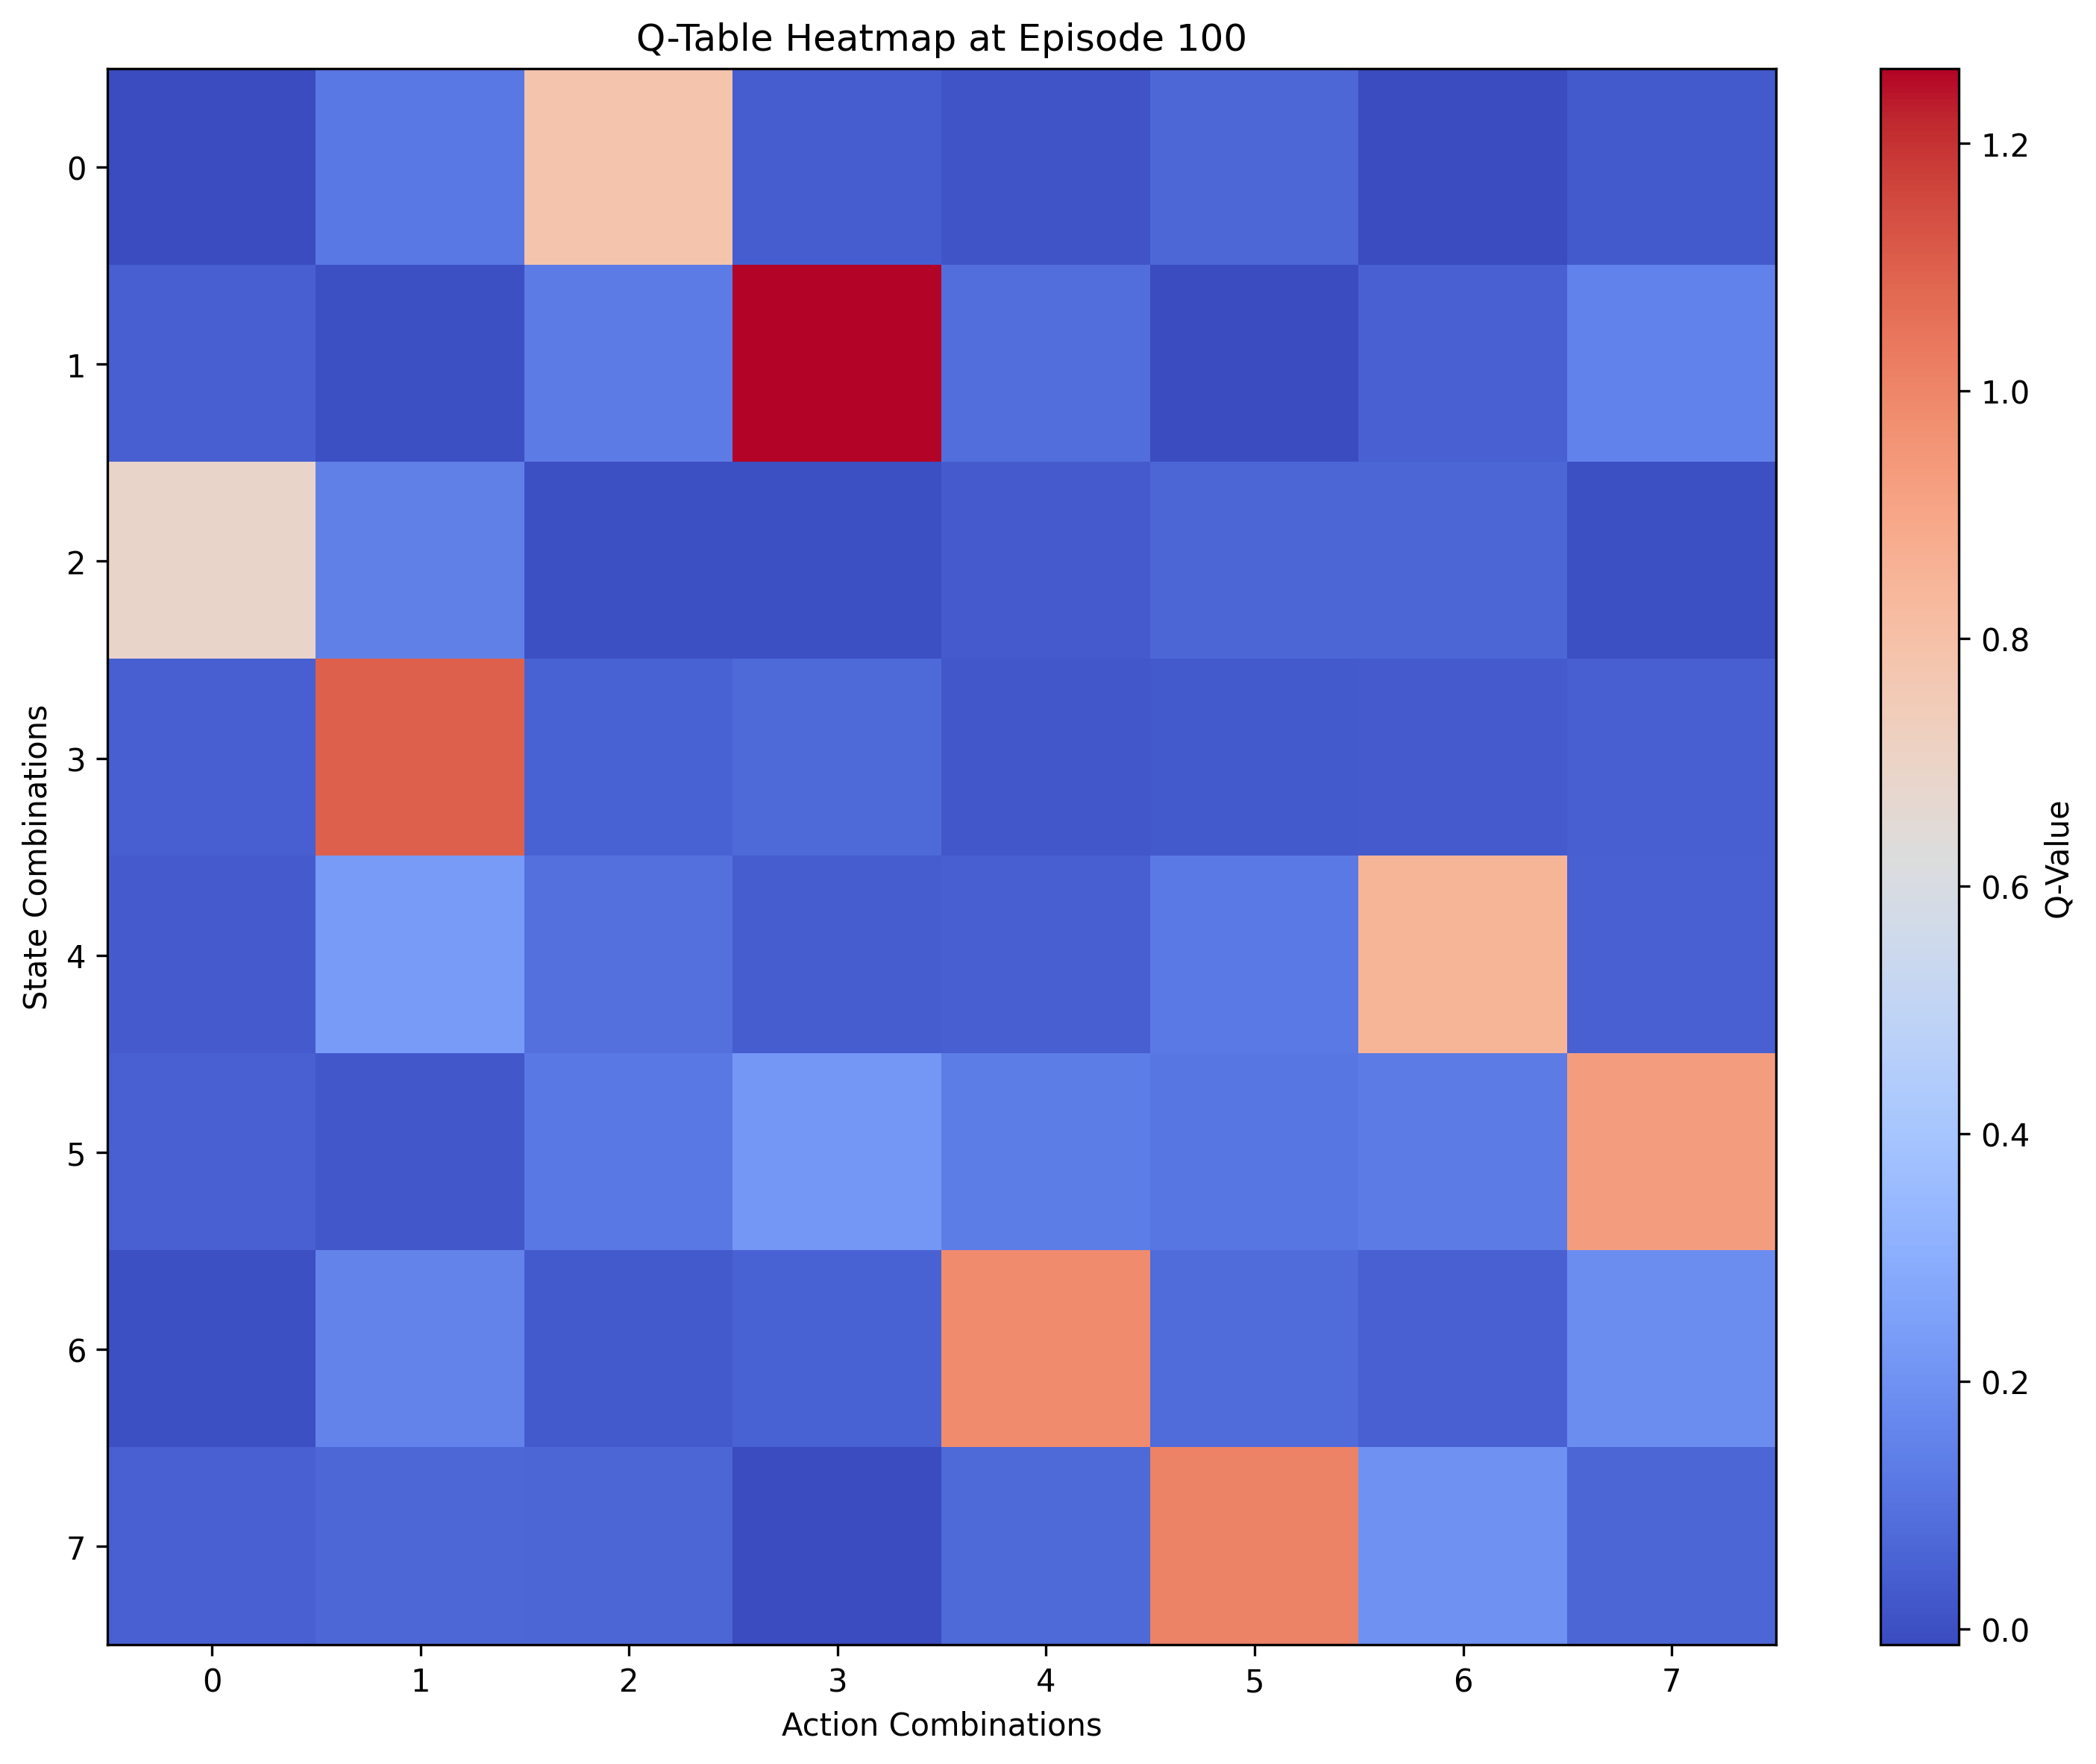
\includegraphics[width=\linewidth]{figure/multi_switch/q_heatmap_episode_100.png}
        \centering (a) Episode 100
    \end{minipage}
    \hfill
    \begin{minipage}{0.45\textwidth}
        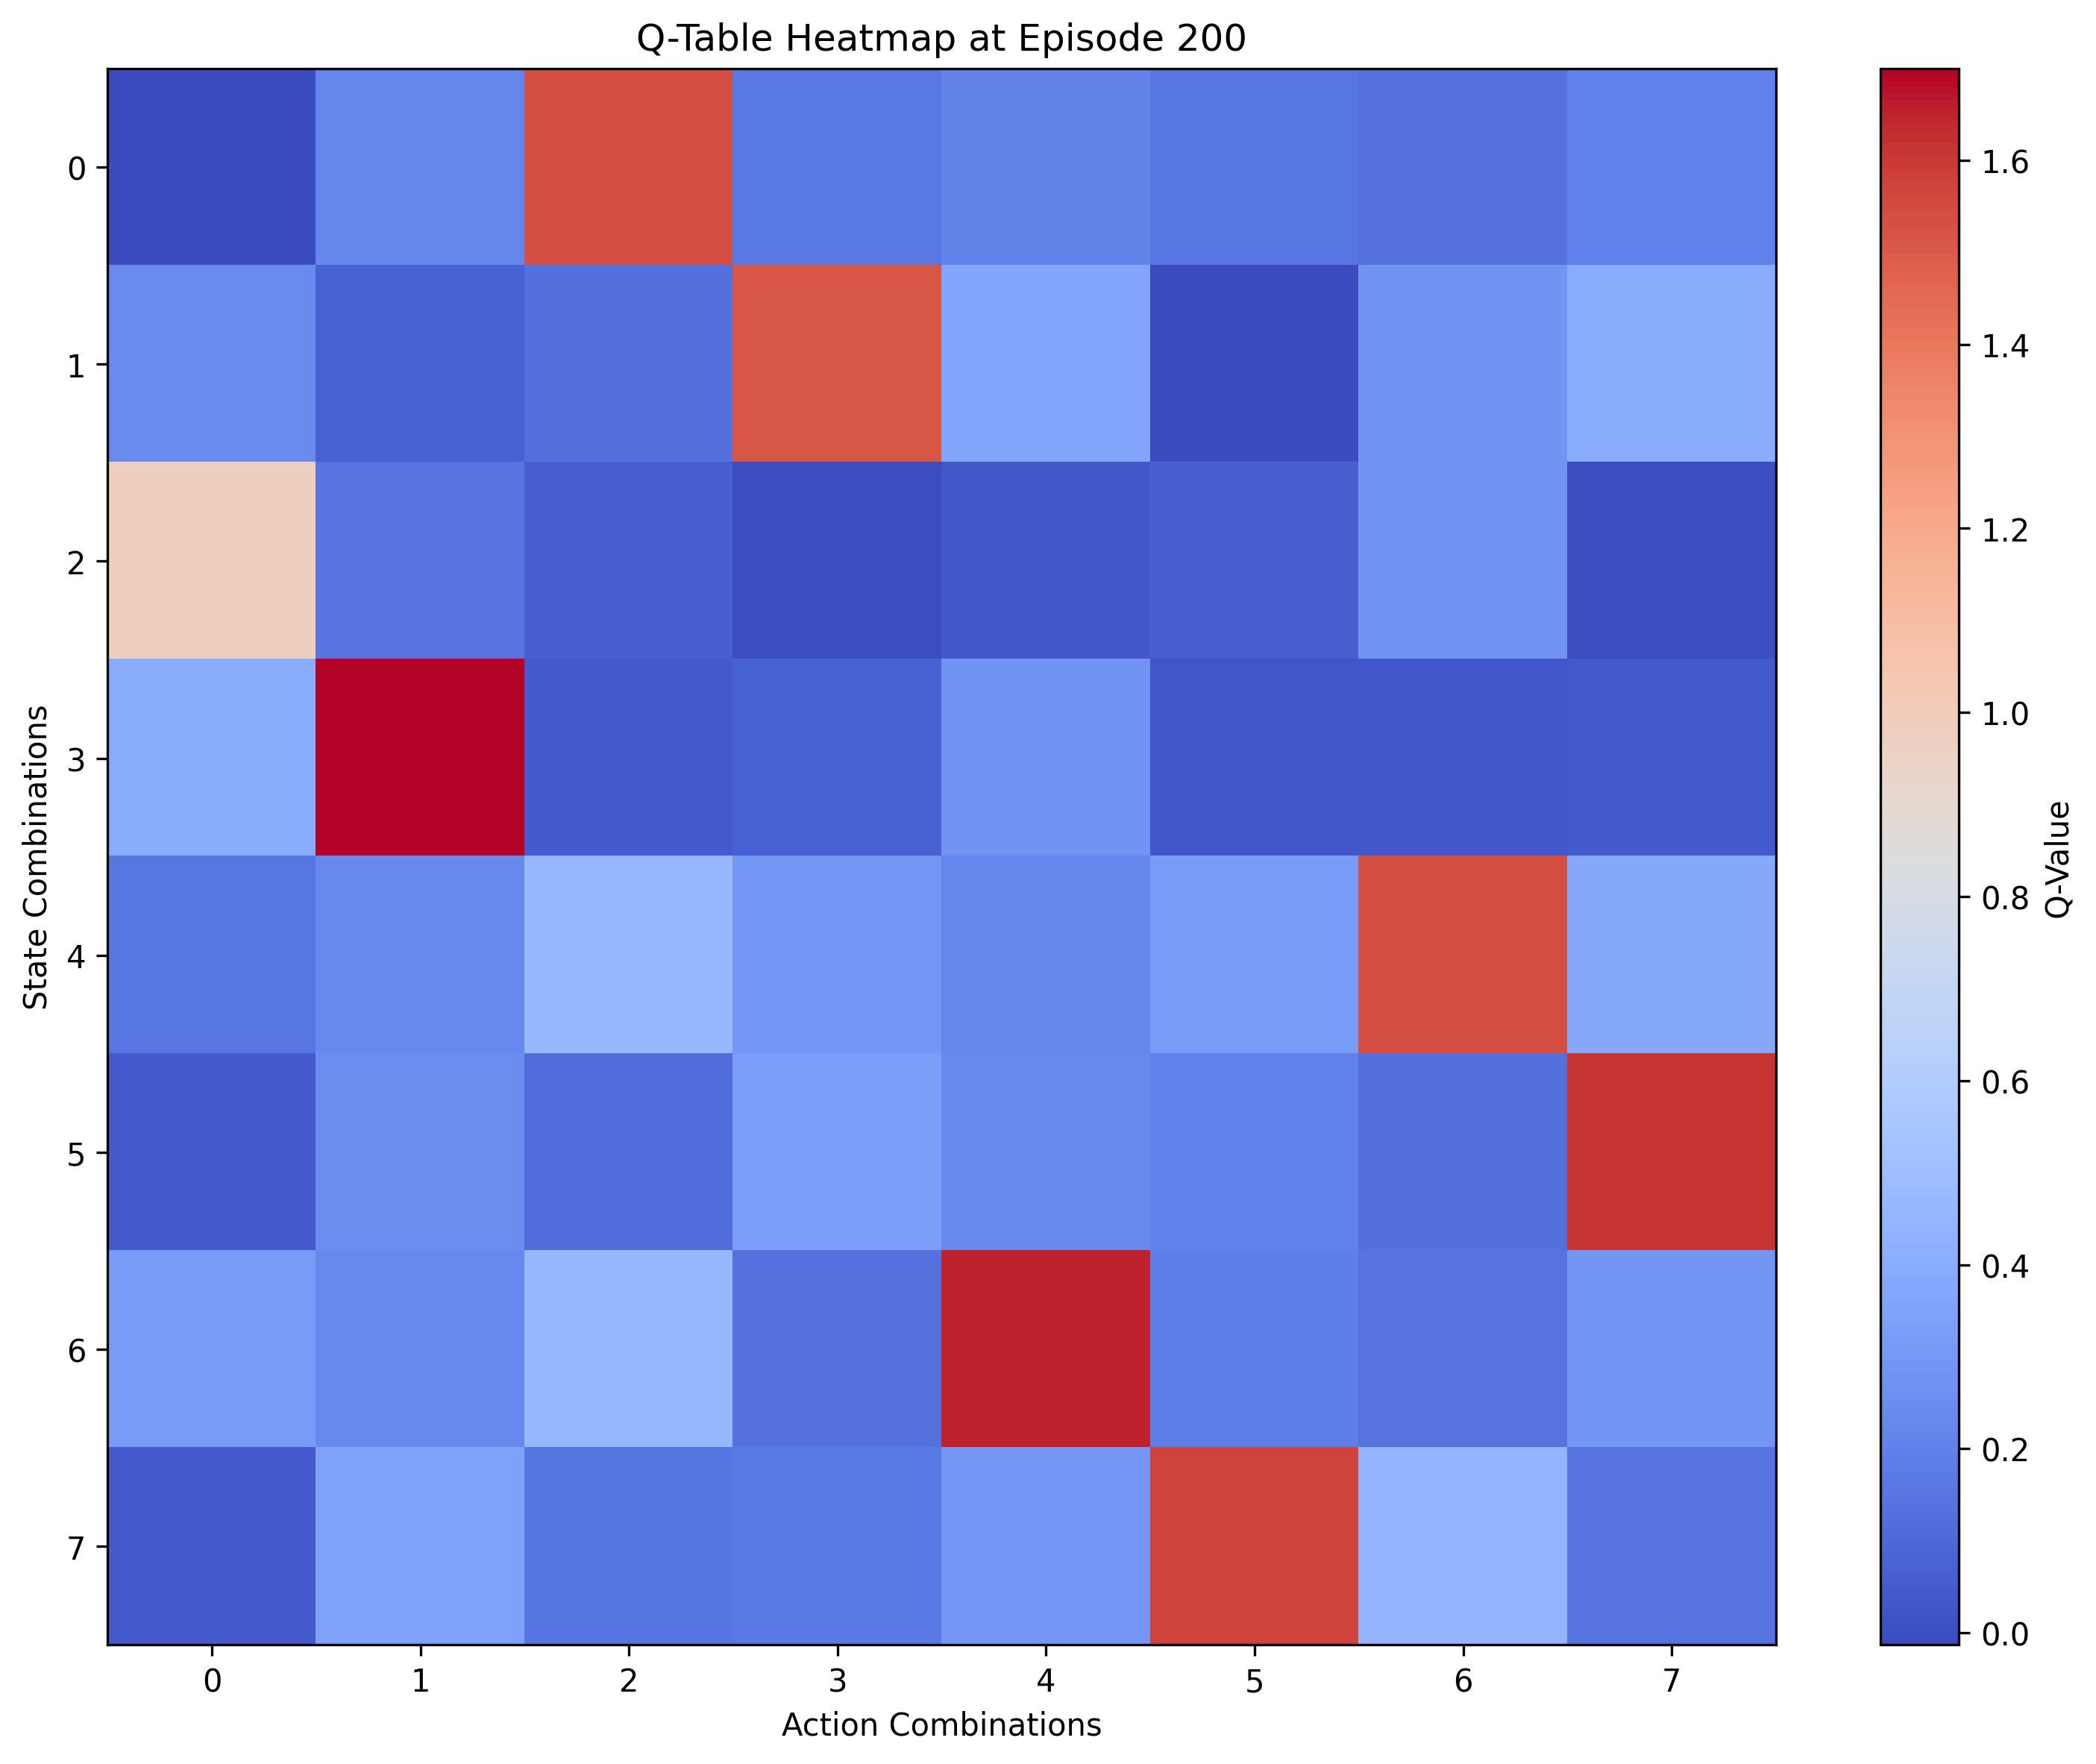
\includegraphics[width=\linewidth]{figure/multi_switch/q_heatmap_episode_200.png}
        \centering (b) Episode 200
    \end{minipage}

    \vspace{0.5em}
    \begin{minipage}{0.45\textwidth}
        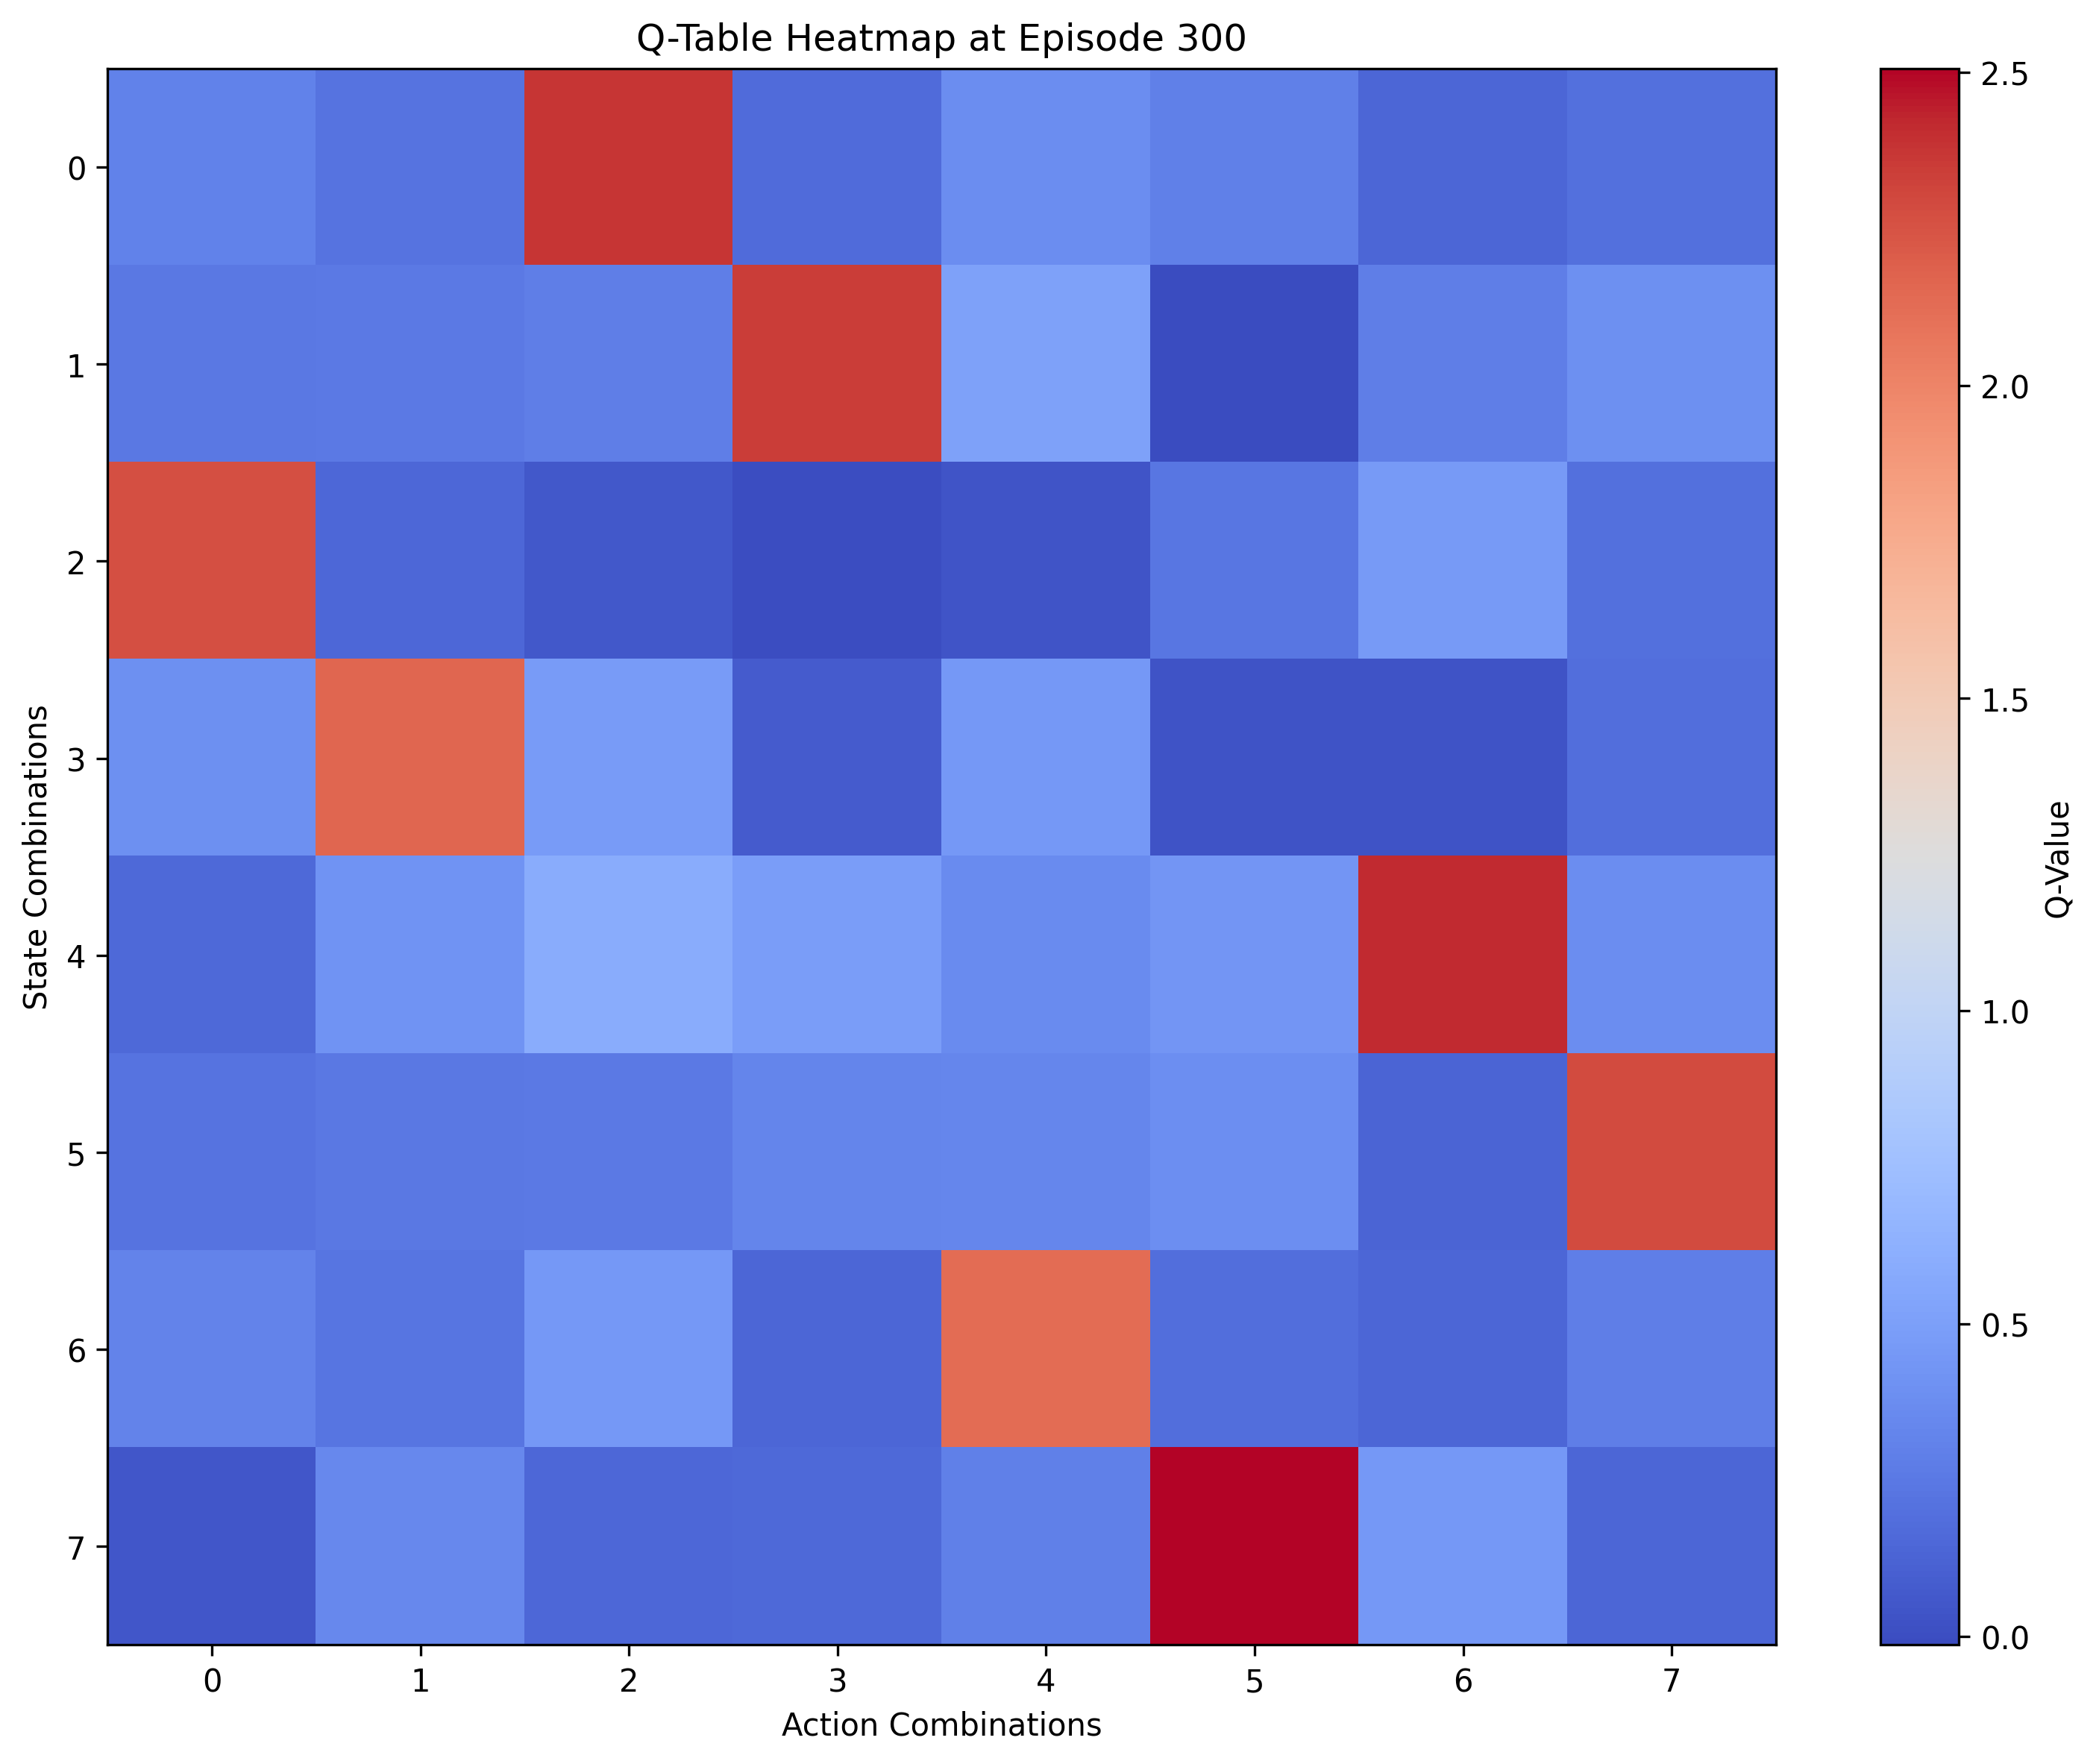
\includegraphics[width=\linewidth]{figure/multi_switch/q_heatmap_episode_300.png}
        \centering (c) Episode 300
    \end{minipage}
    \hfill
    \begin{minipage}{0.45\textwidth}
        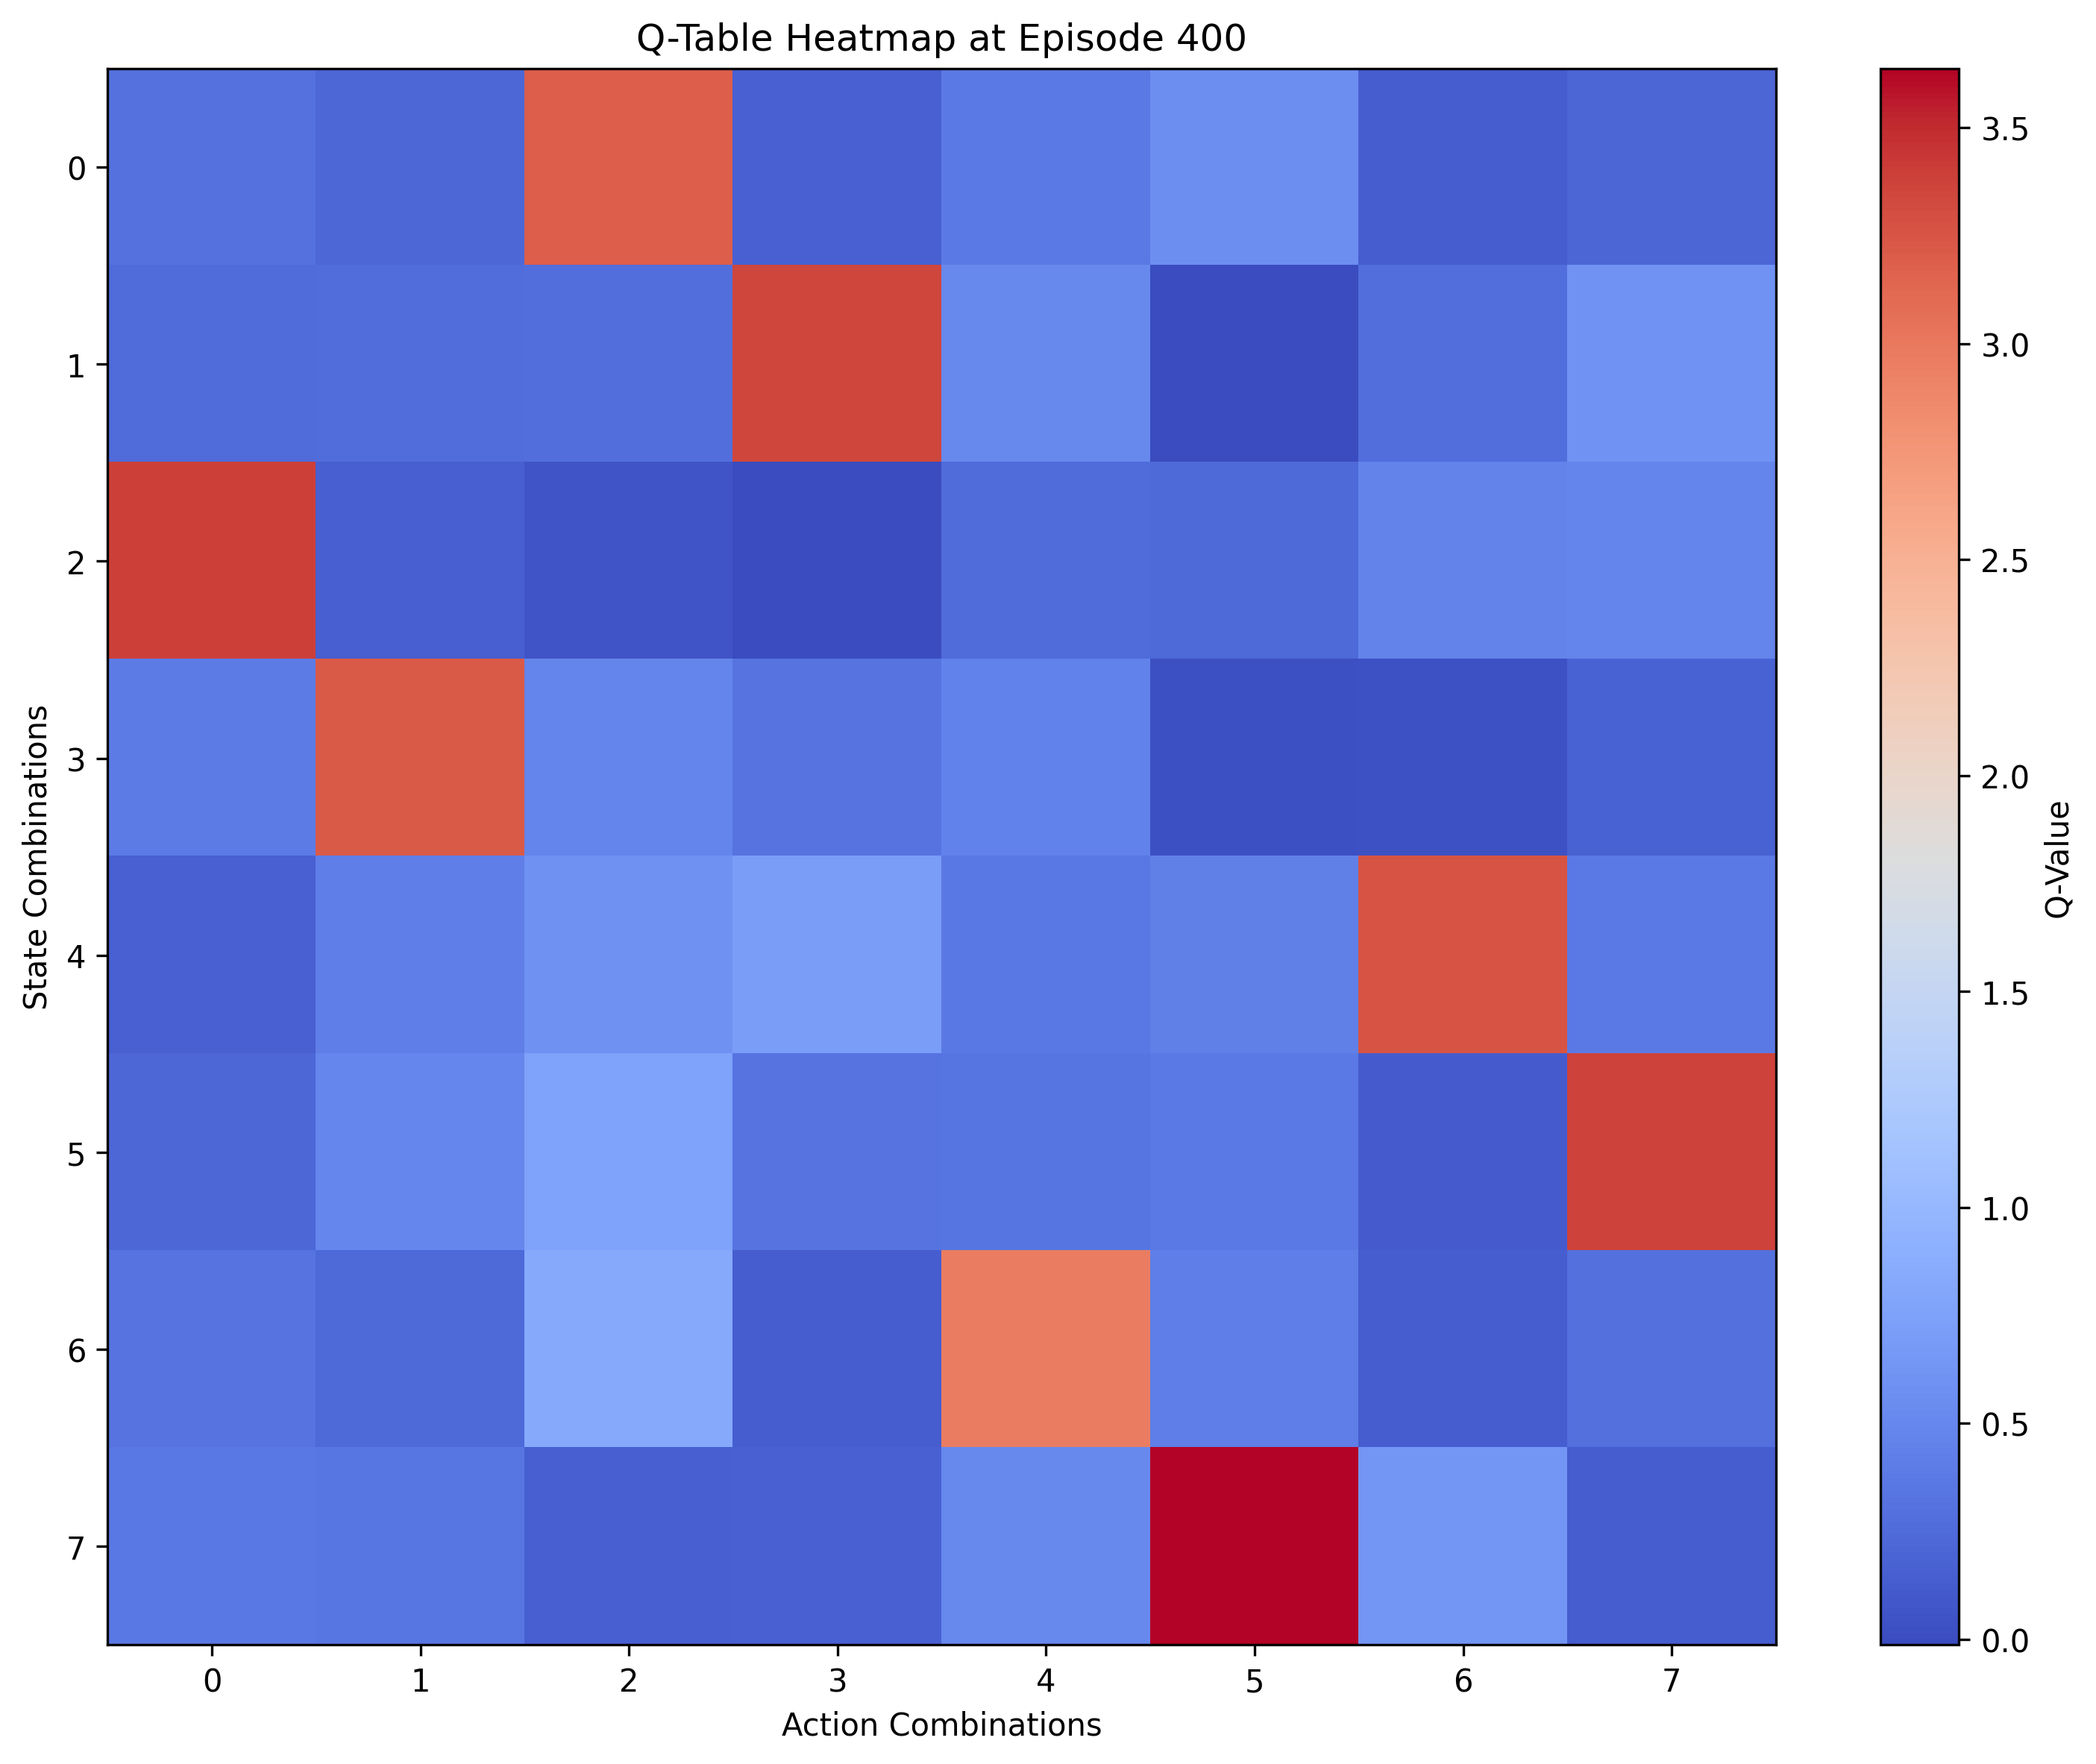
\includegraphics[width=\linewidth]{figure/multi_switch/q_heatmap_episode_400.png}
        \centering (d) Episode 400
    \end{minipage}

    \vspace{0.5em}
    \begin{minipage}{0.45\textwidth}
        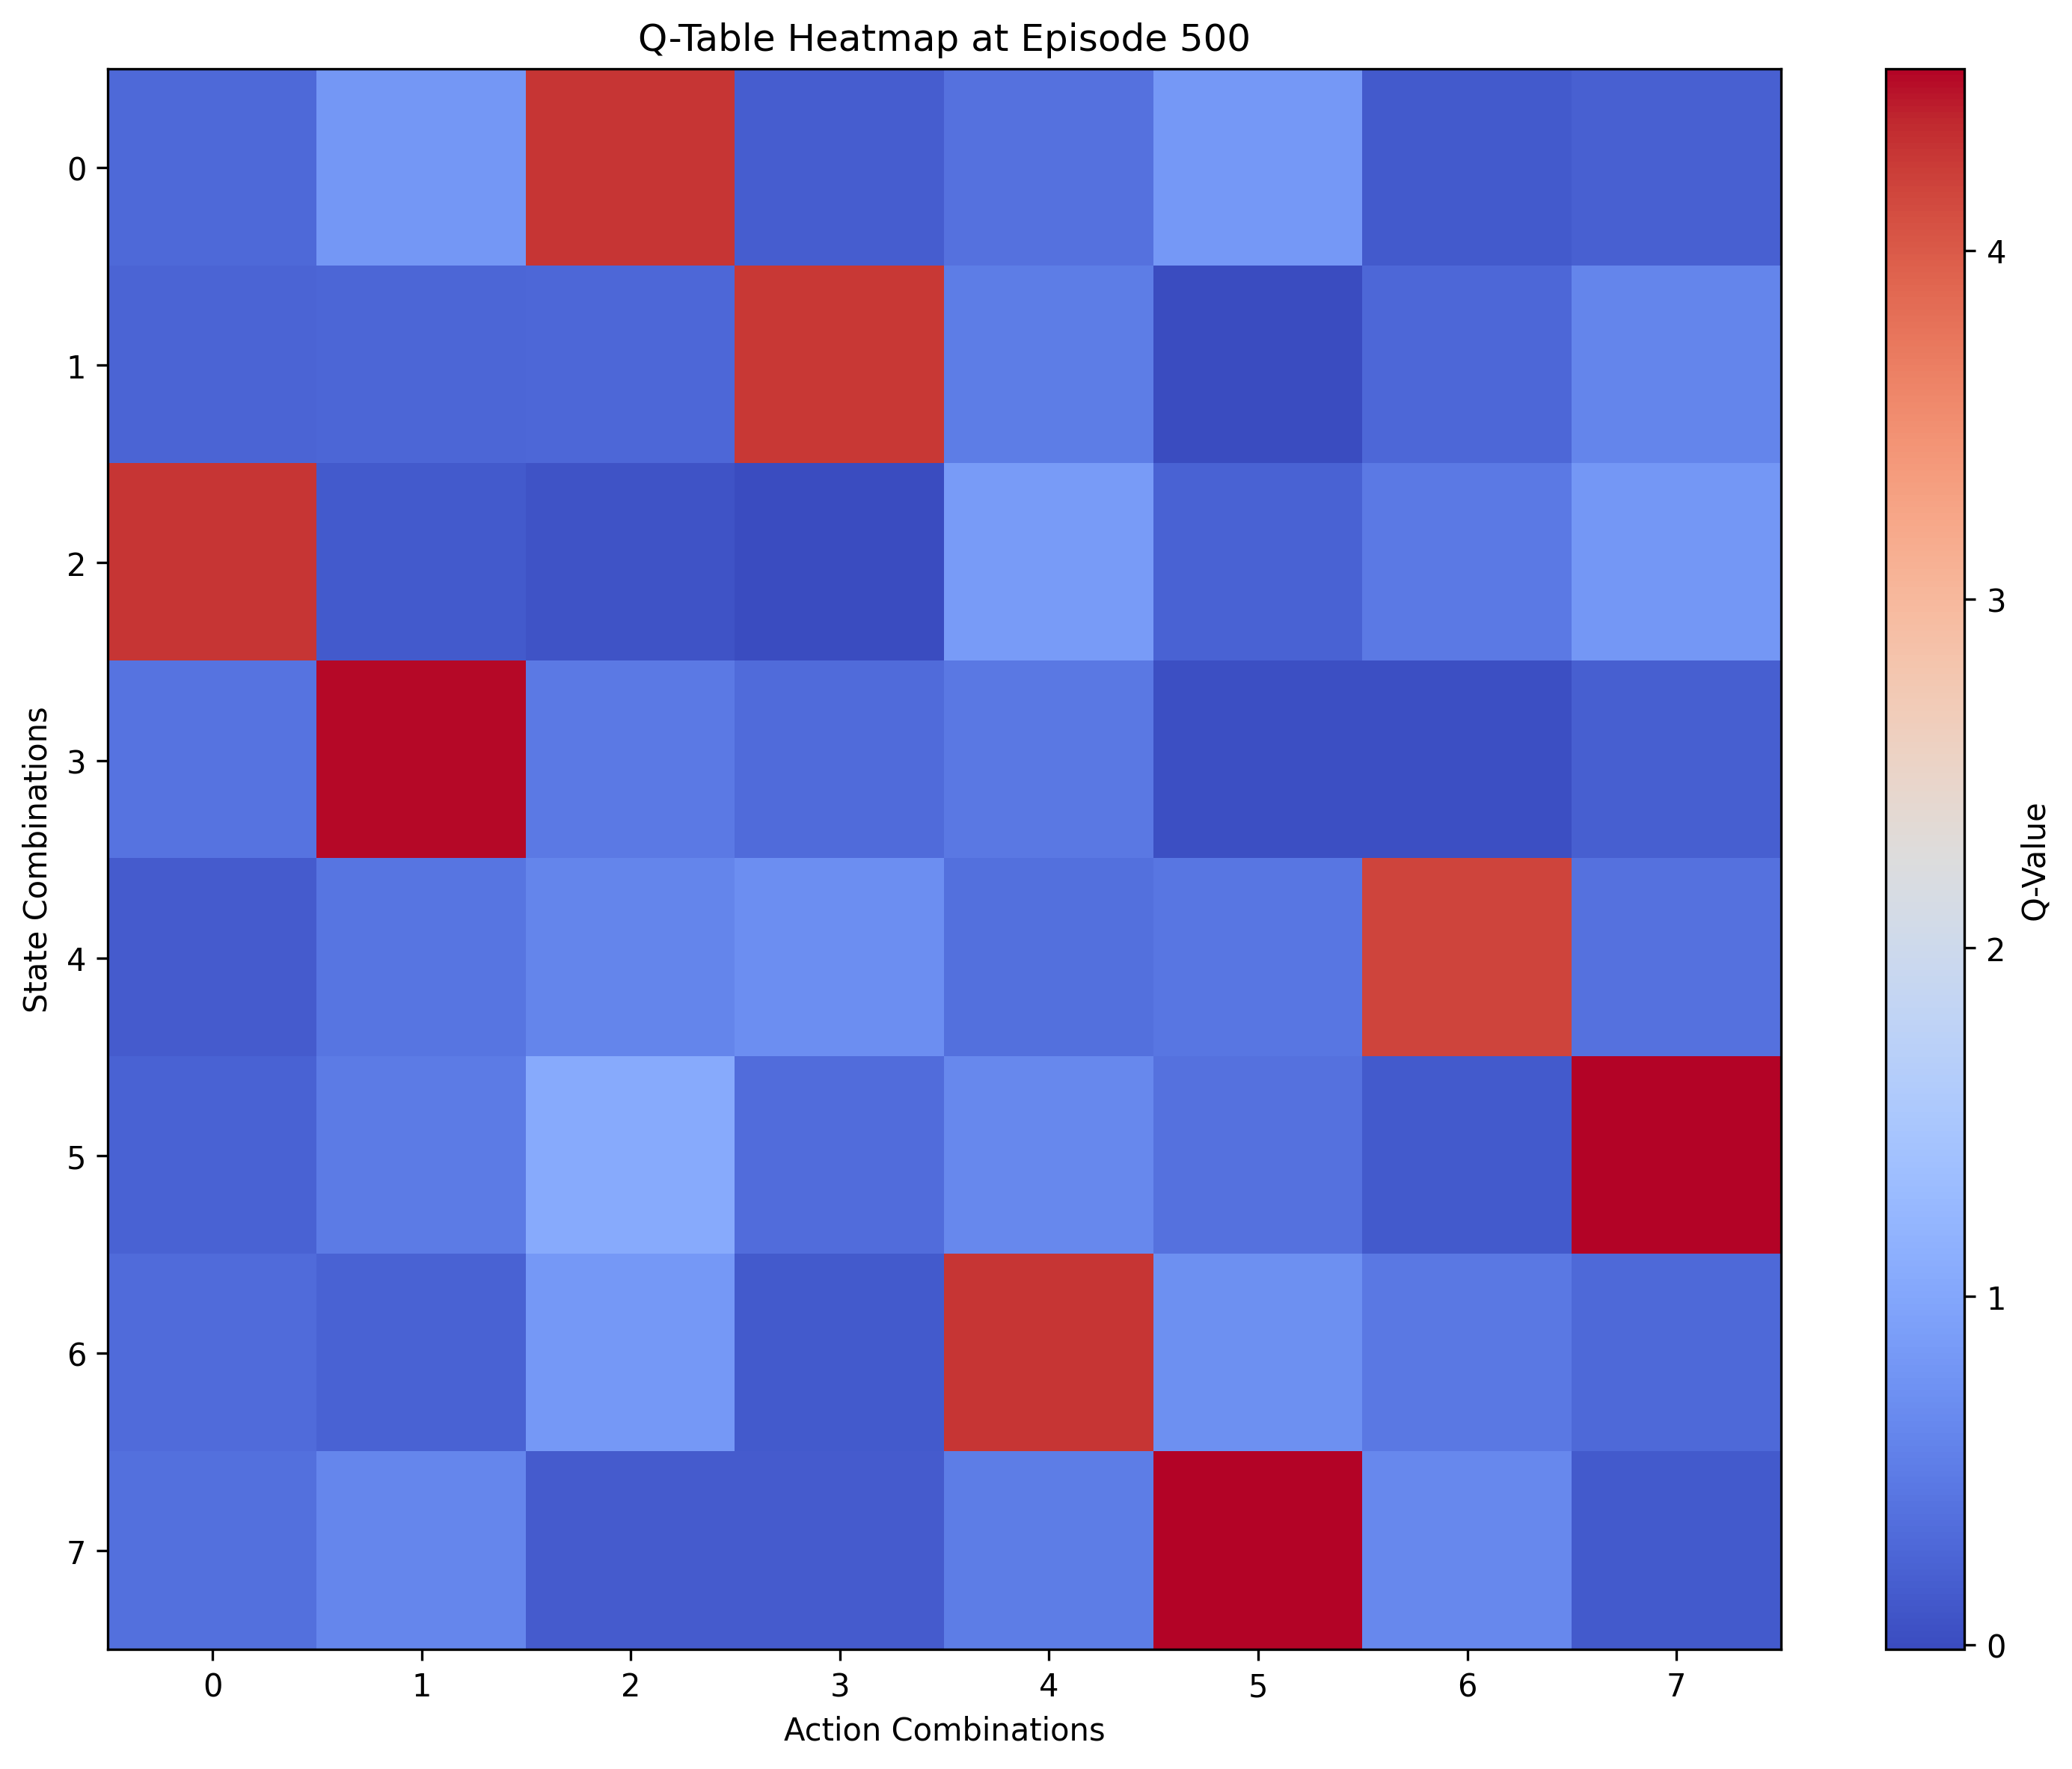
\includegraphics[width=\linewidth]{figure/multi_switch/q_heatmap_episode_500.png}
        \centering (e)Episode 500
    \end{minipage}
    \hfill
    \begin{minipage}{0.45\textwidth}
        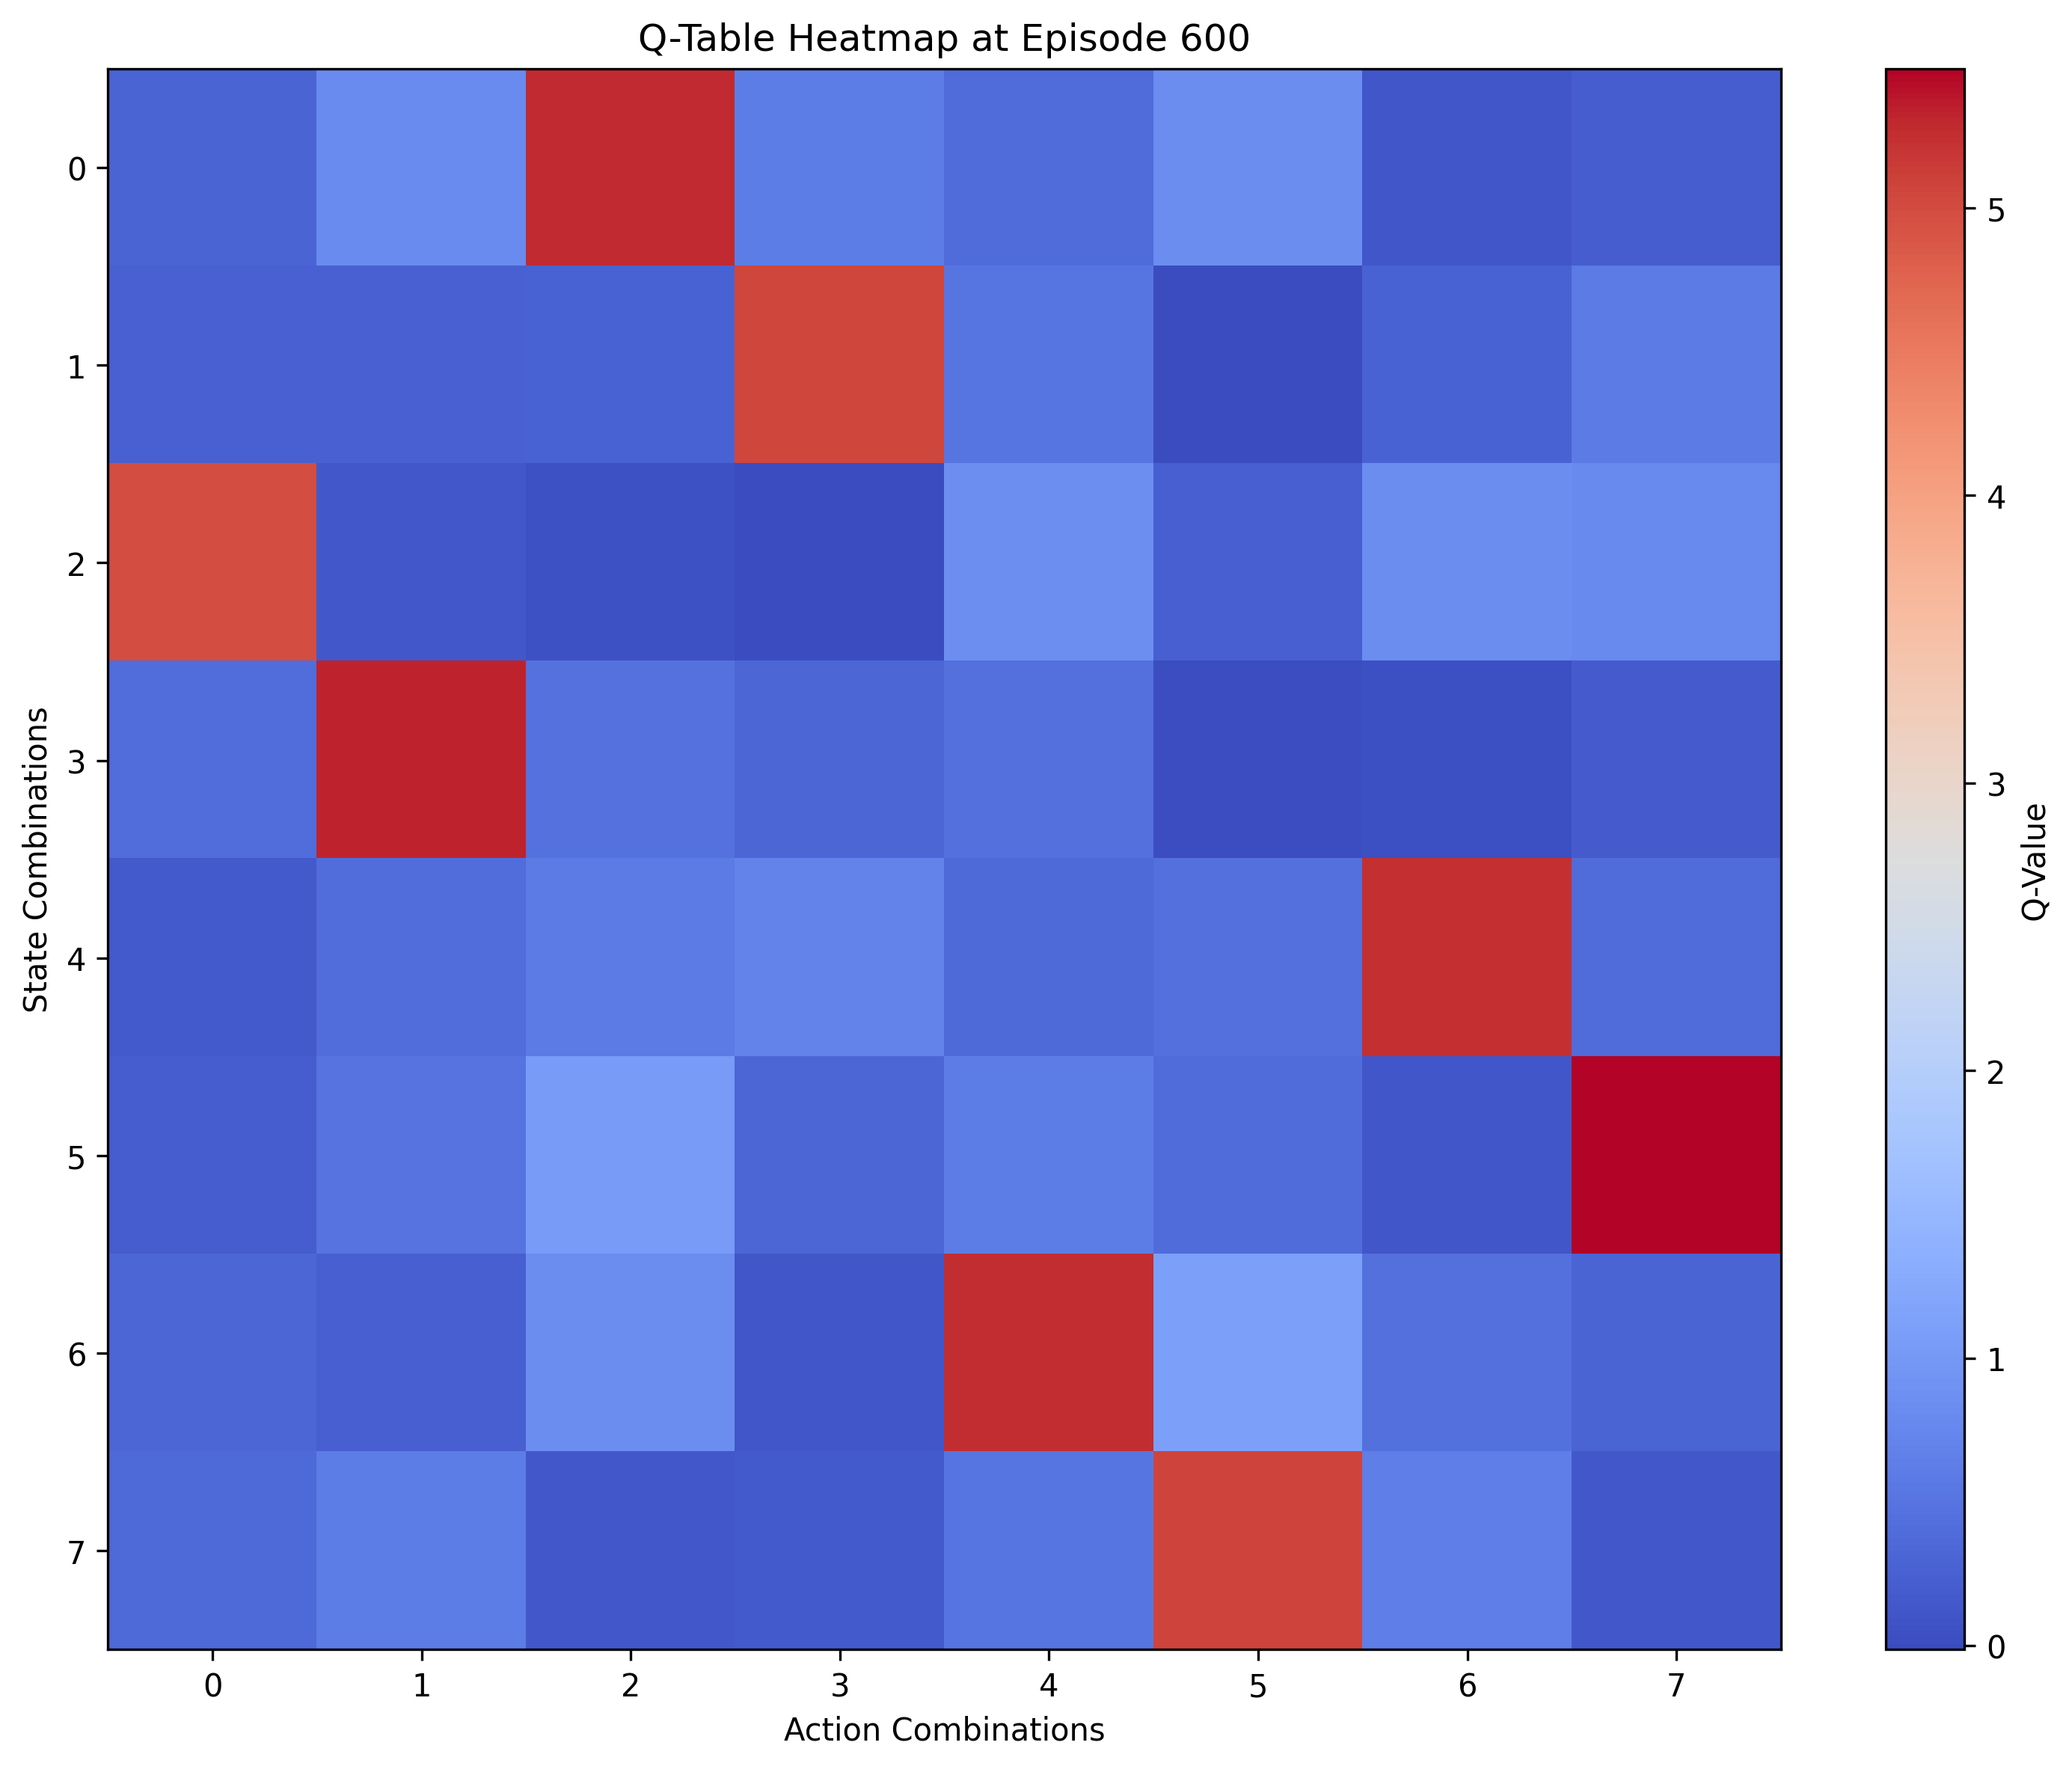
\includegraphics[width=\linewidth]{figure/multi_switch/q_heatmap_episode_600.png}
        \centering (f) Episode 600
    \end{minipage}

    \caption{训练过程中 \(Q\) 值热力图的演化(Episode 100–600,每 100 回合)}
    \label{fig:qvalue_snapshots}
\end{figure}

\begin{figure}[htbp]
    \ContinuedFloat
    \centering
    
    \begin{minipage}{0.45\textwidth}
        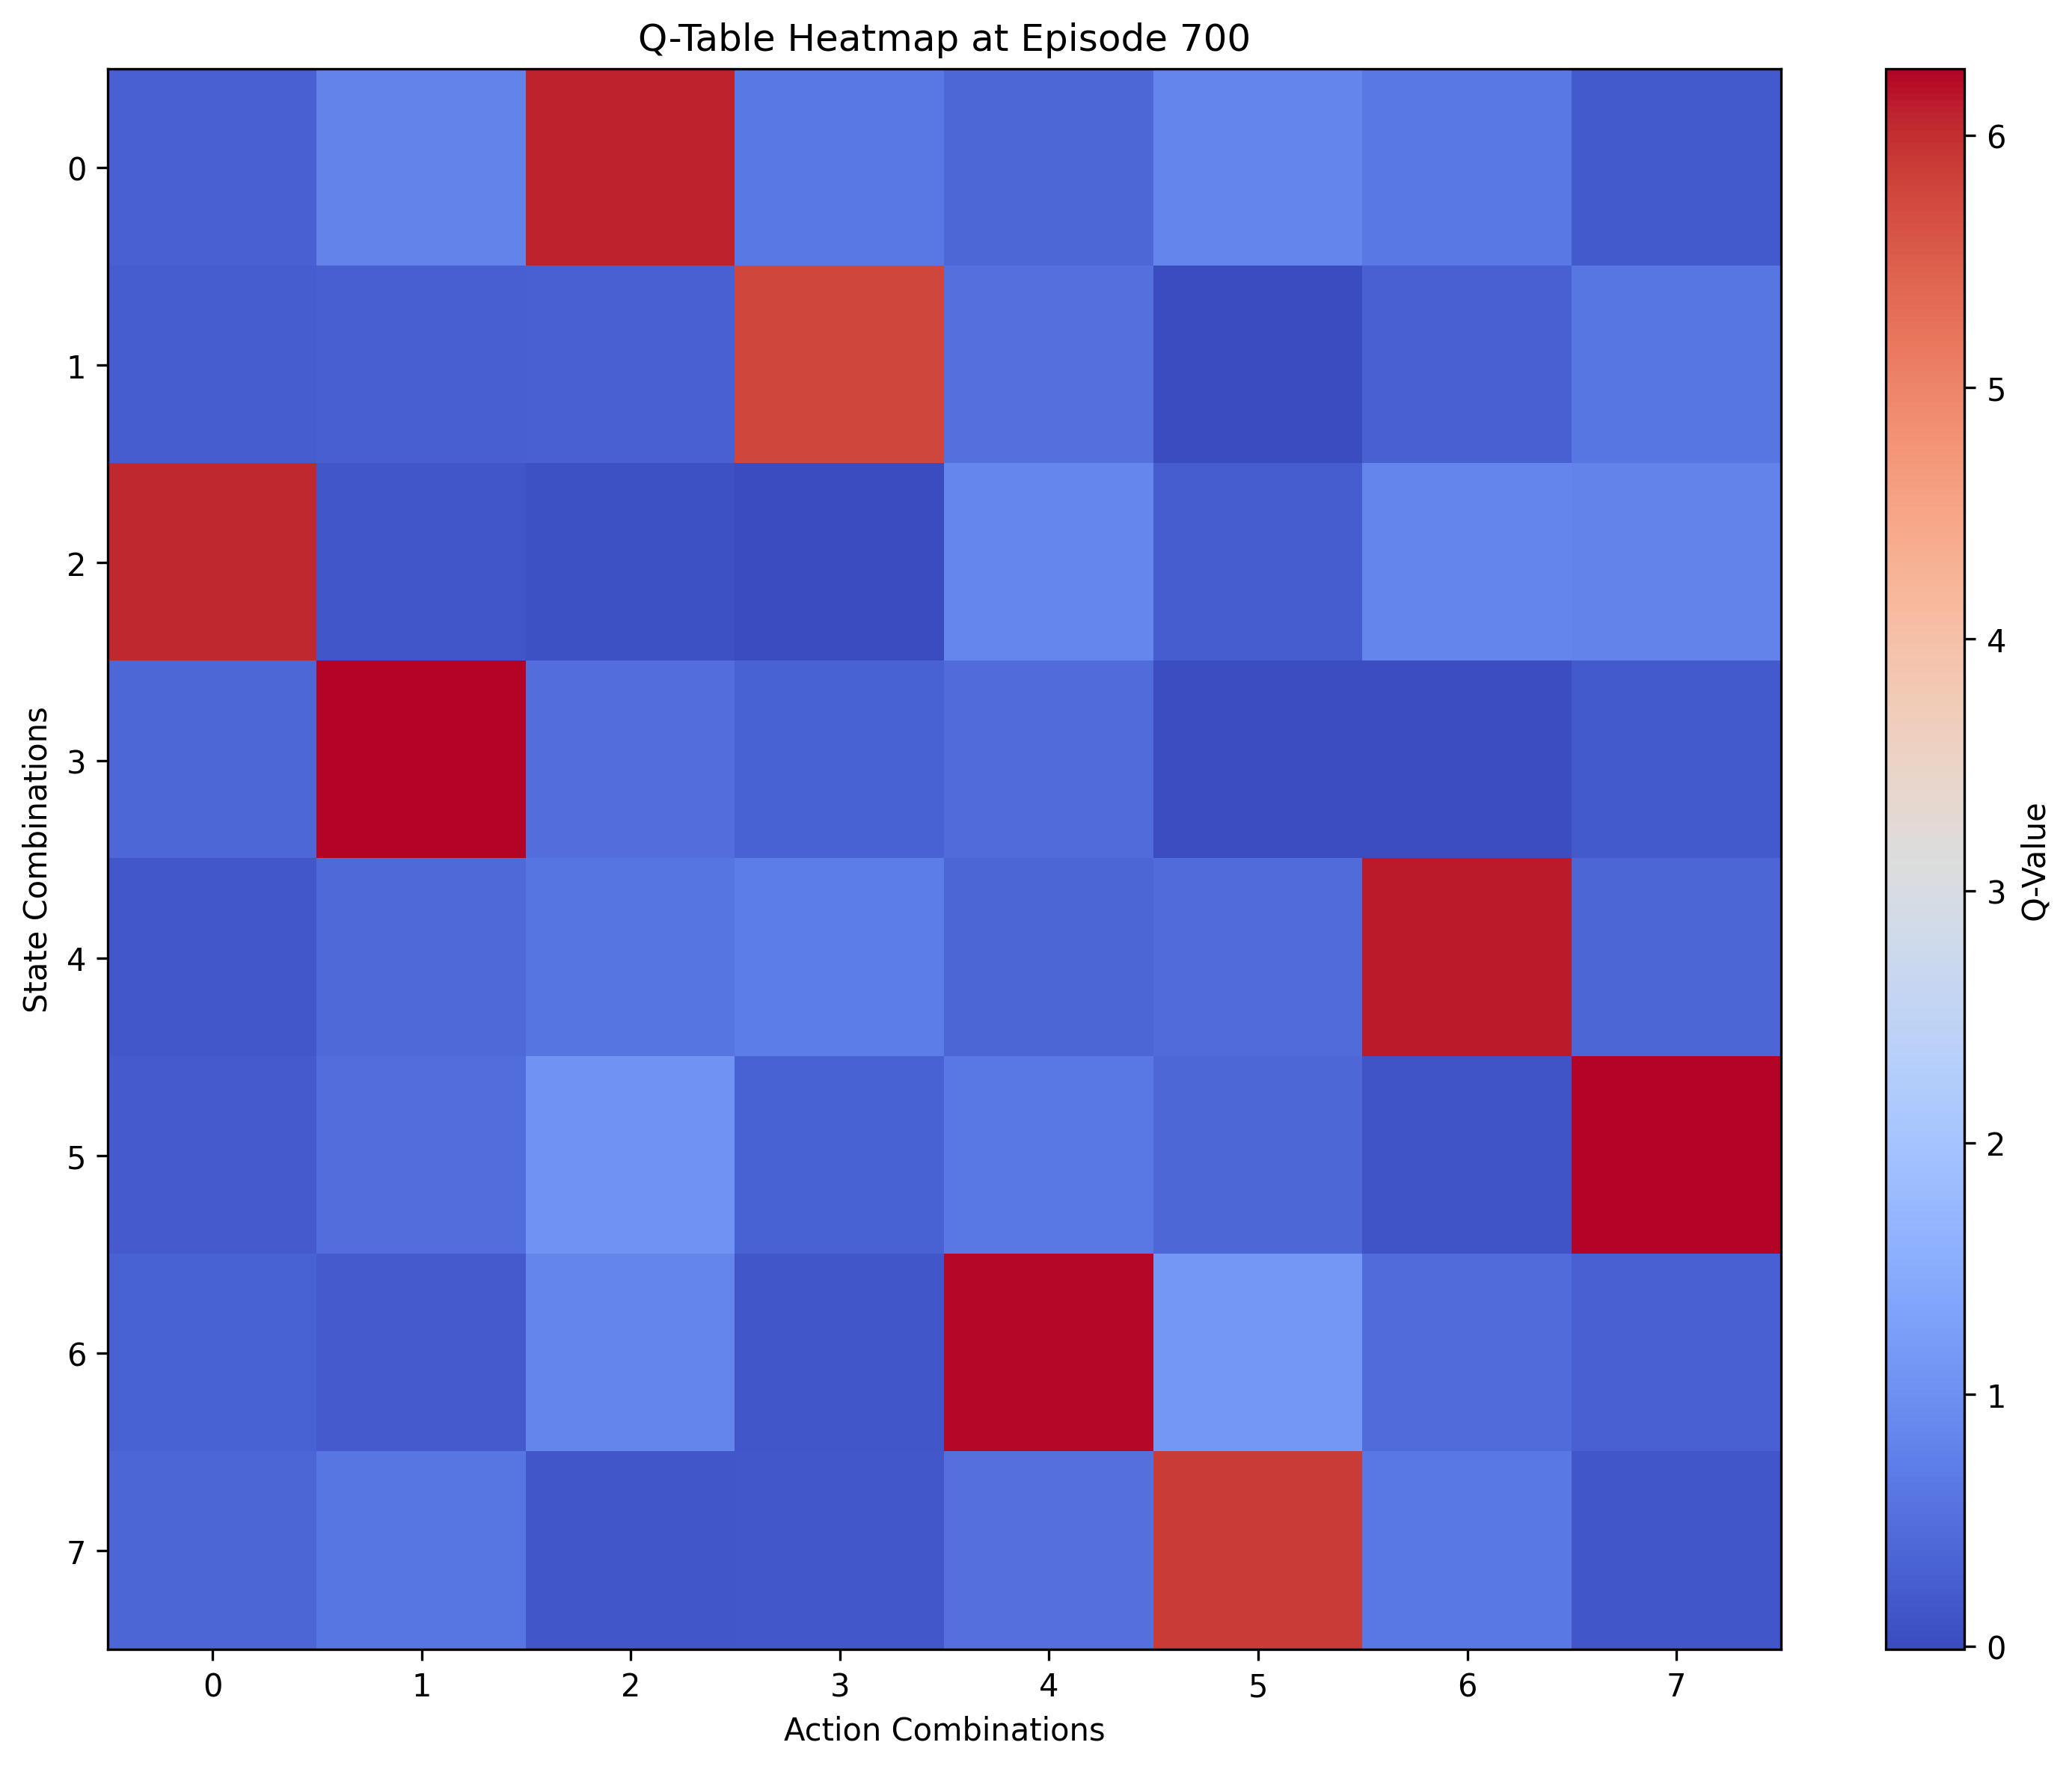
\includegraphics[width=\linewidth]{figure/multi_switch/q_heatmap_episode_700.png}
        \centering (g) Episode 700
    \end{minipage}
    \hfill
    \begin{minipage}{0.45\textwidth}
        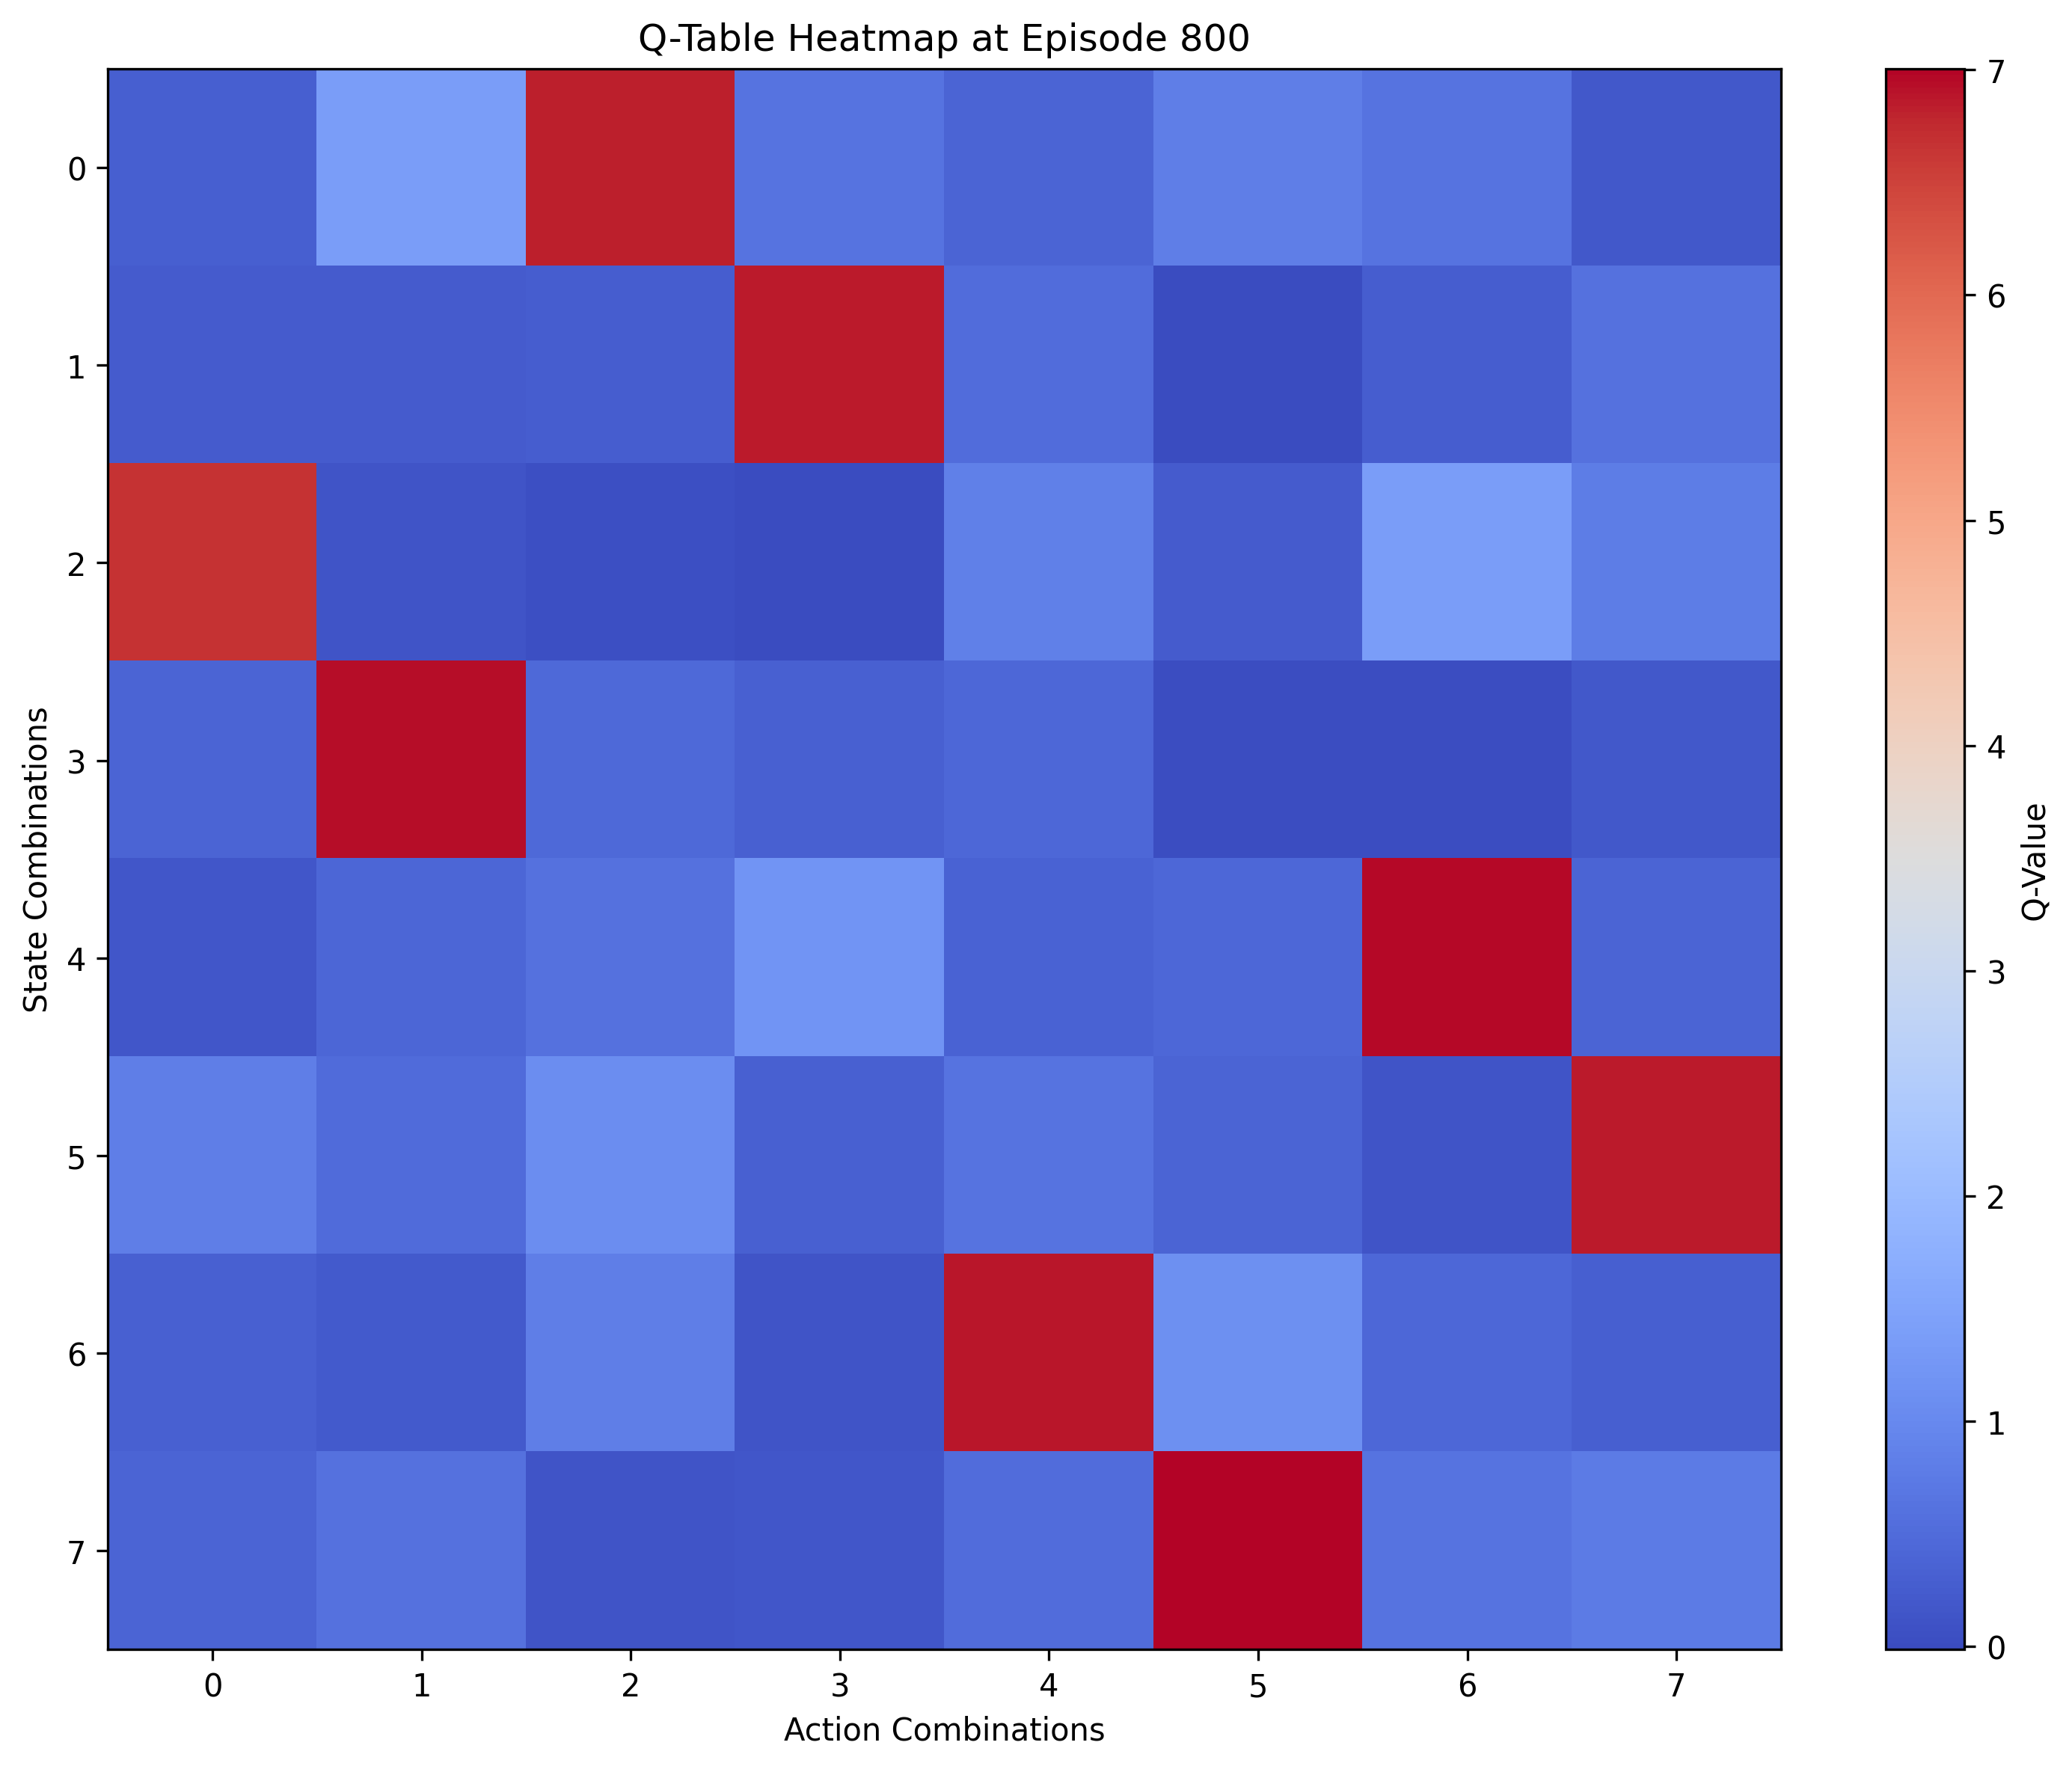
\includegraphics[width=\linewidth]{figure/multi_switch/q_heatmap_episode_800.png}
        \centering (h) Episode 800
    \end{minipage}

    \vspace{0.5em}
    \begin{minipage}{0.45\textwidth}
        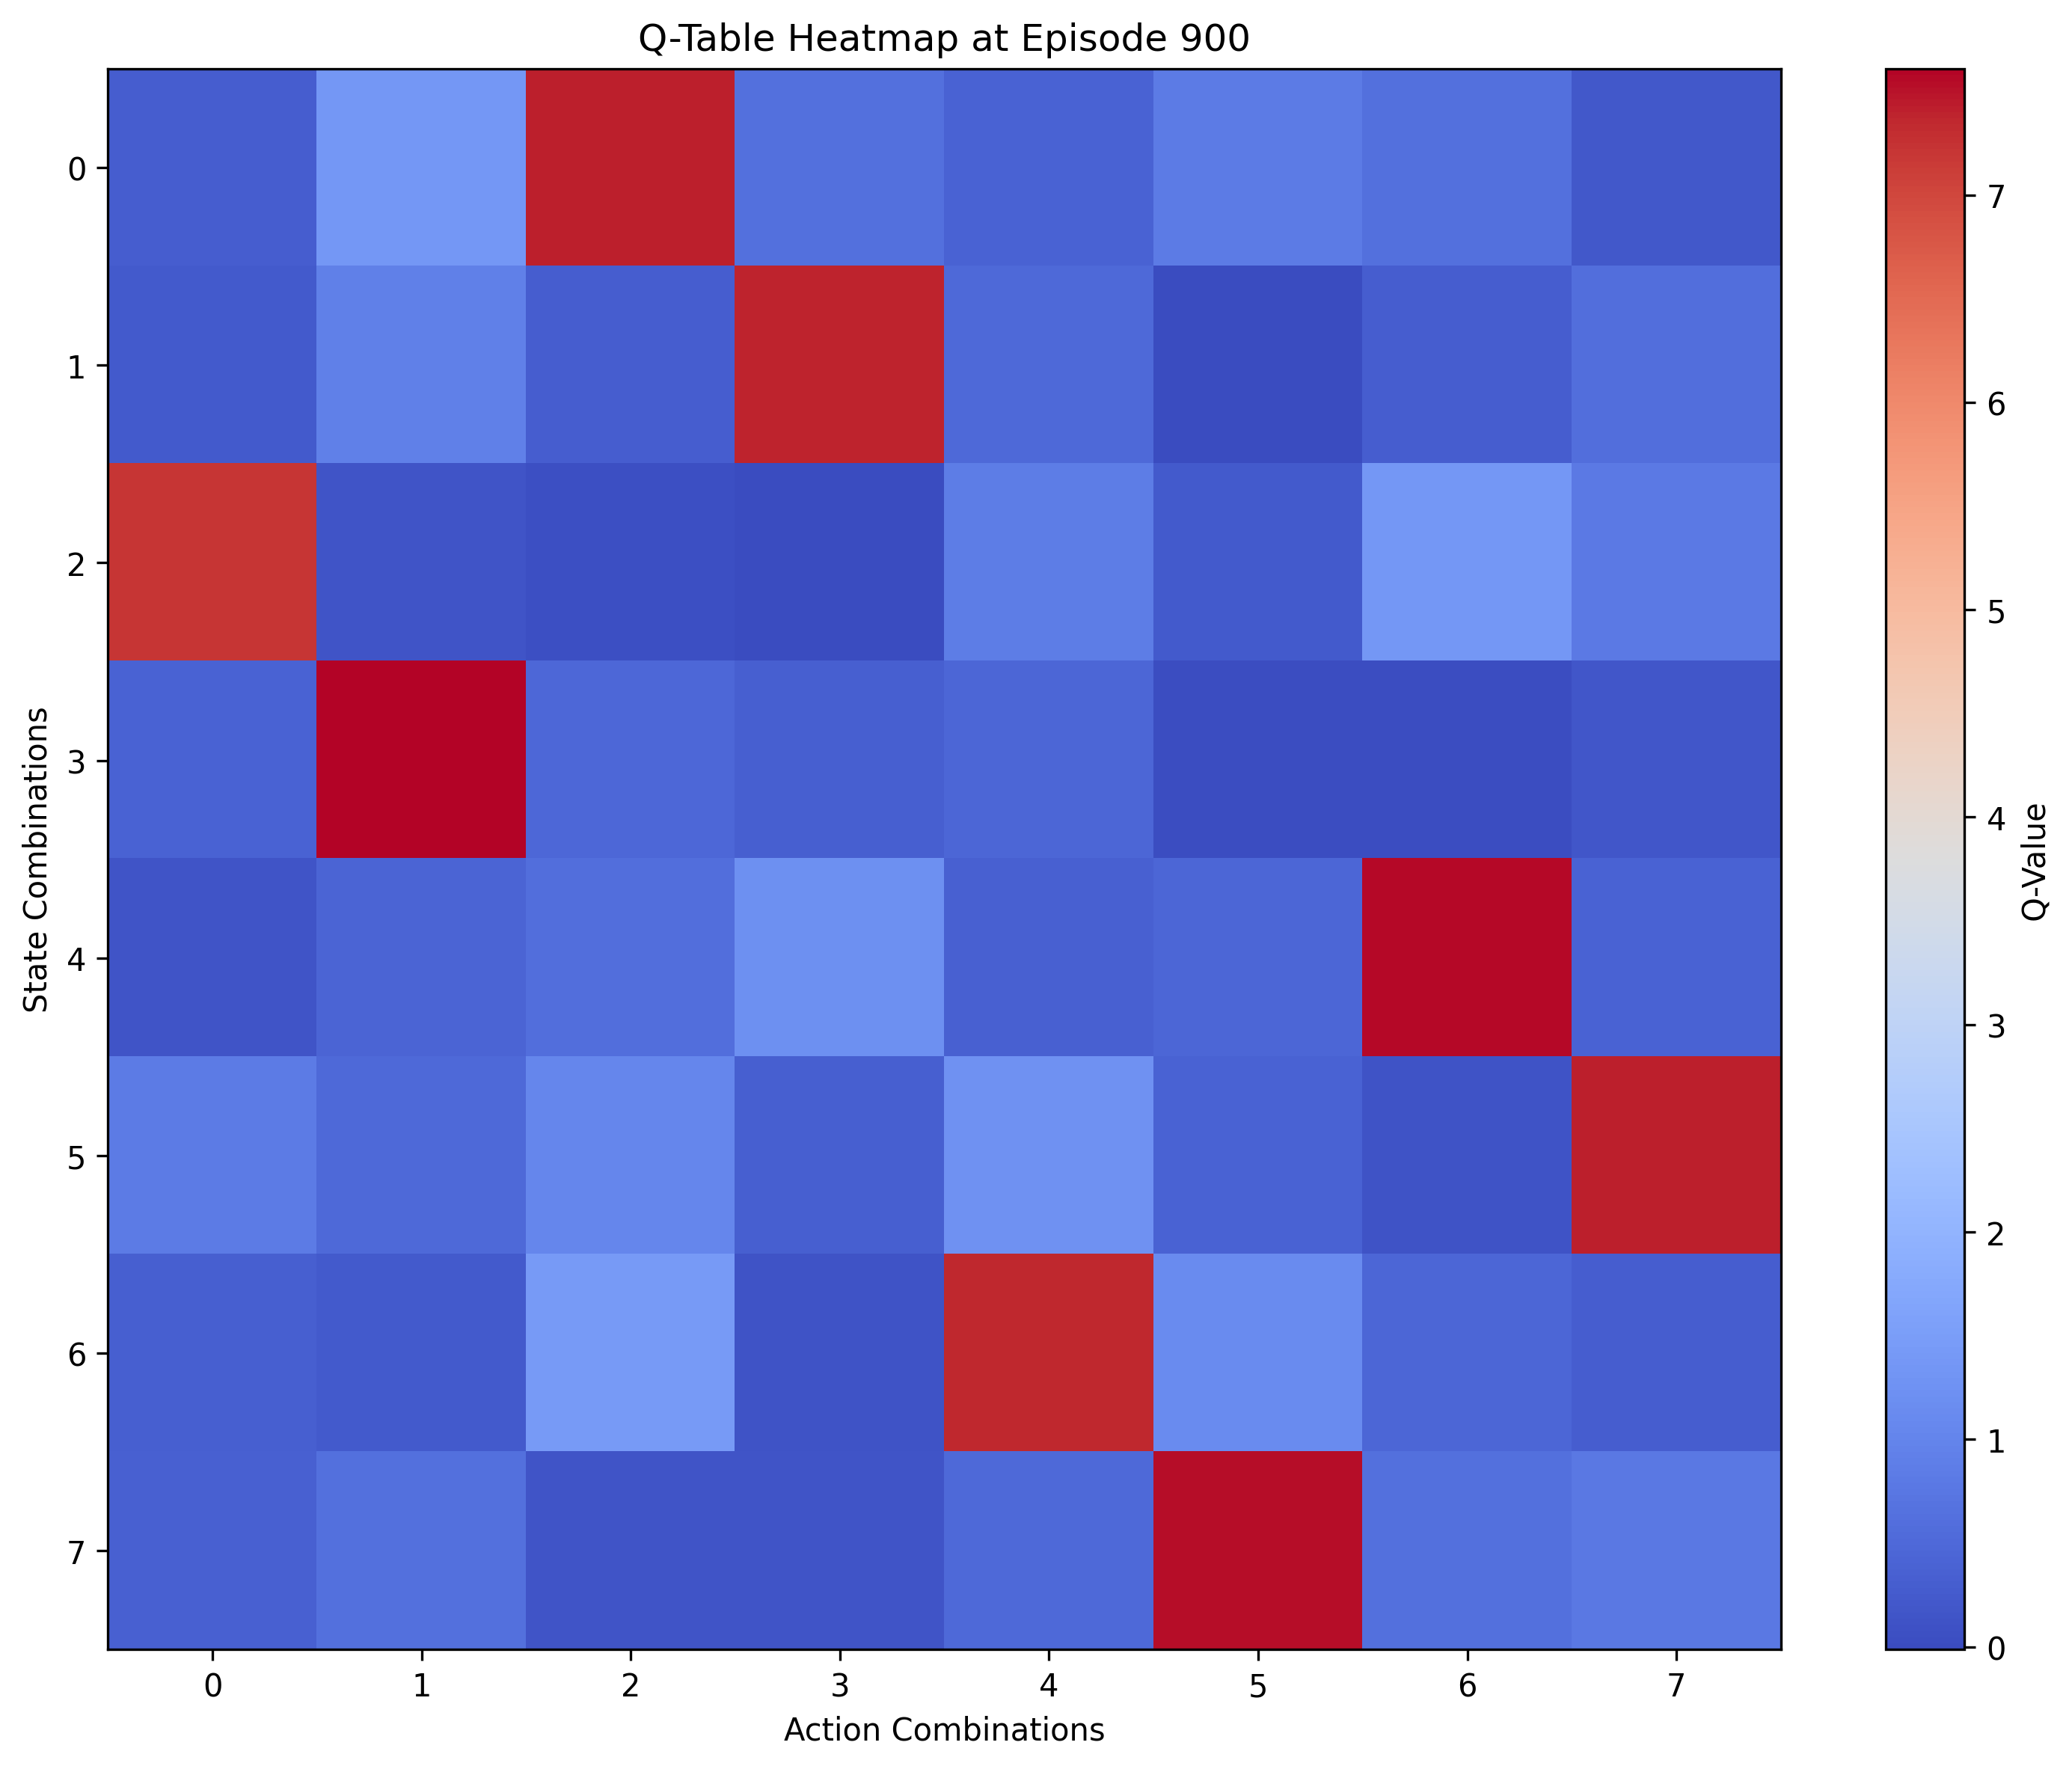
\includegraphics[width=\linewidth]{figure/multi_switch/q_heatmap_episode_900.png}
        \centering (i) Episode 900
    \end{minipage}
    \hfill
    \begin{minipage}{0.45\textwidth}
        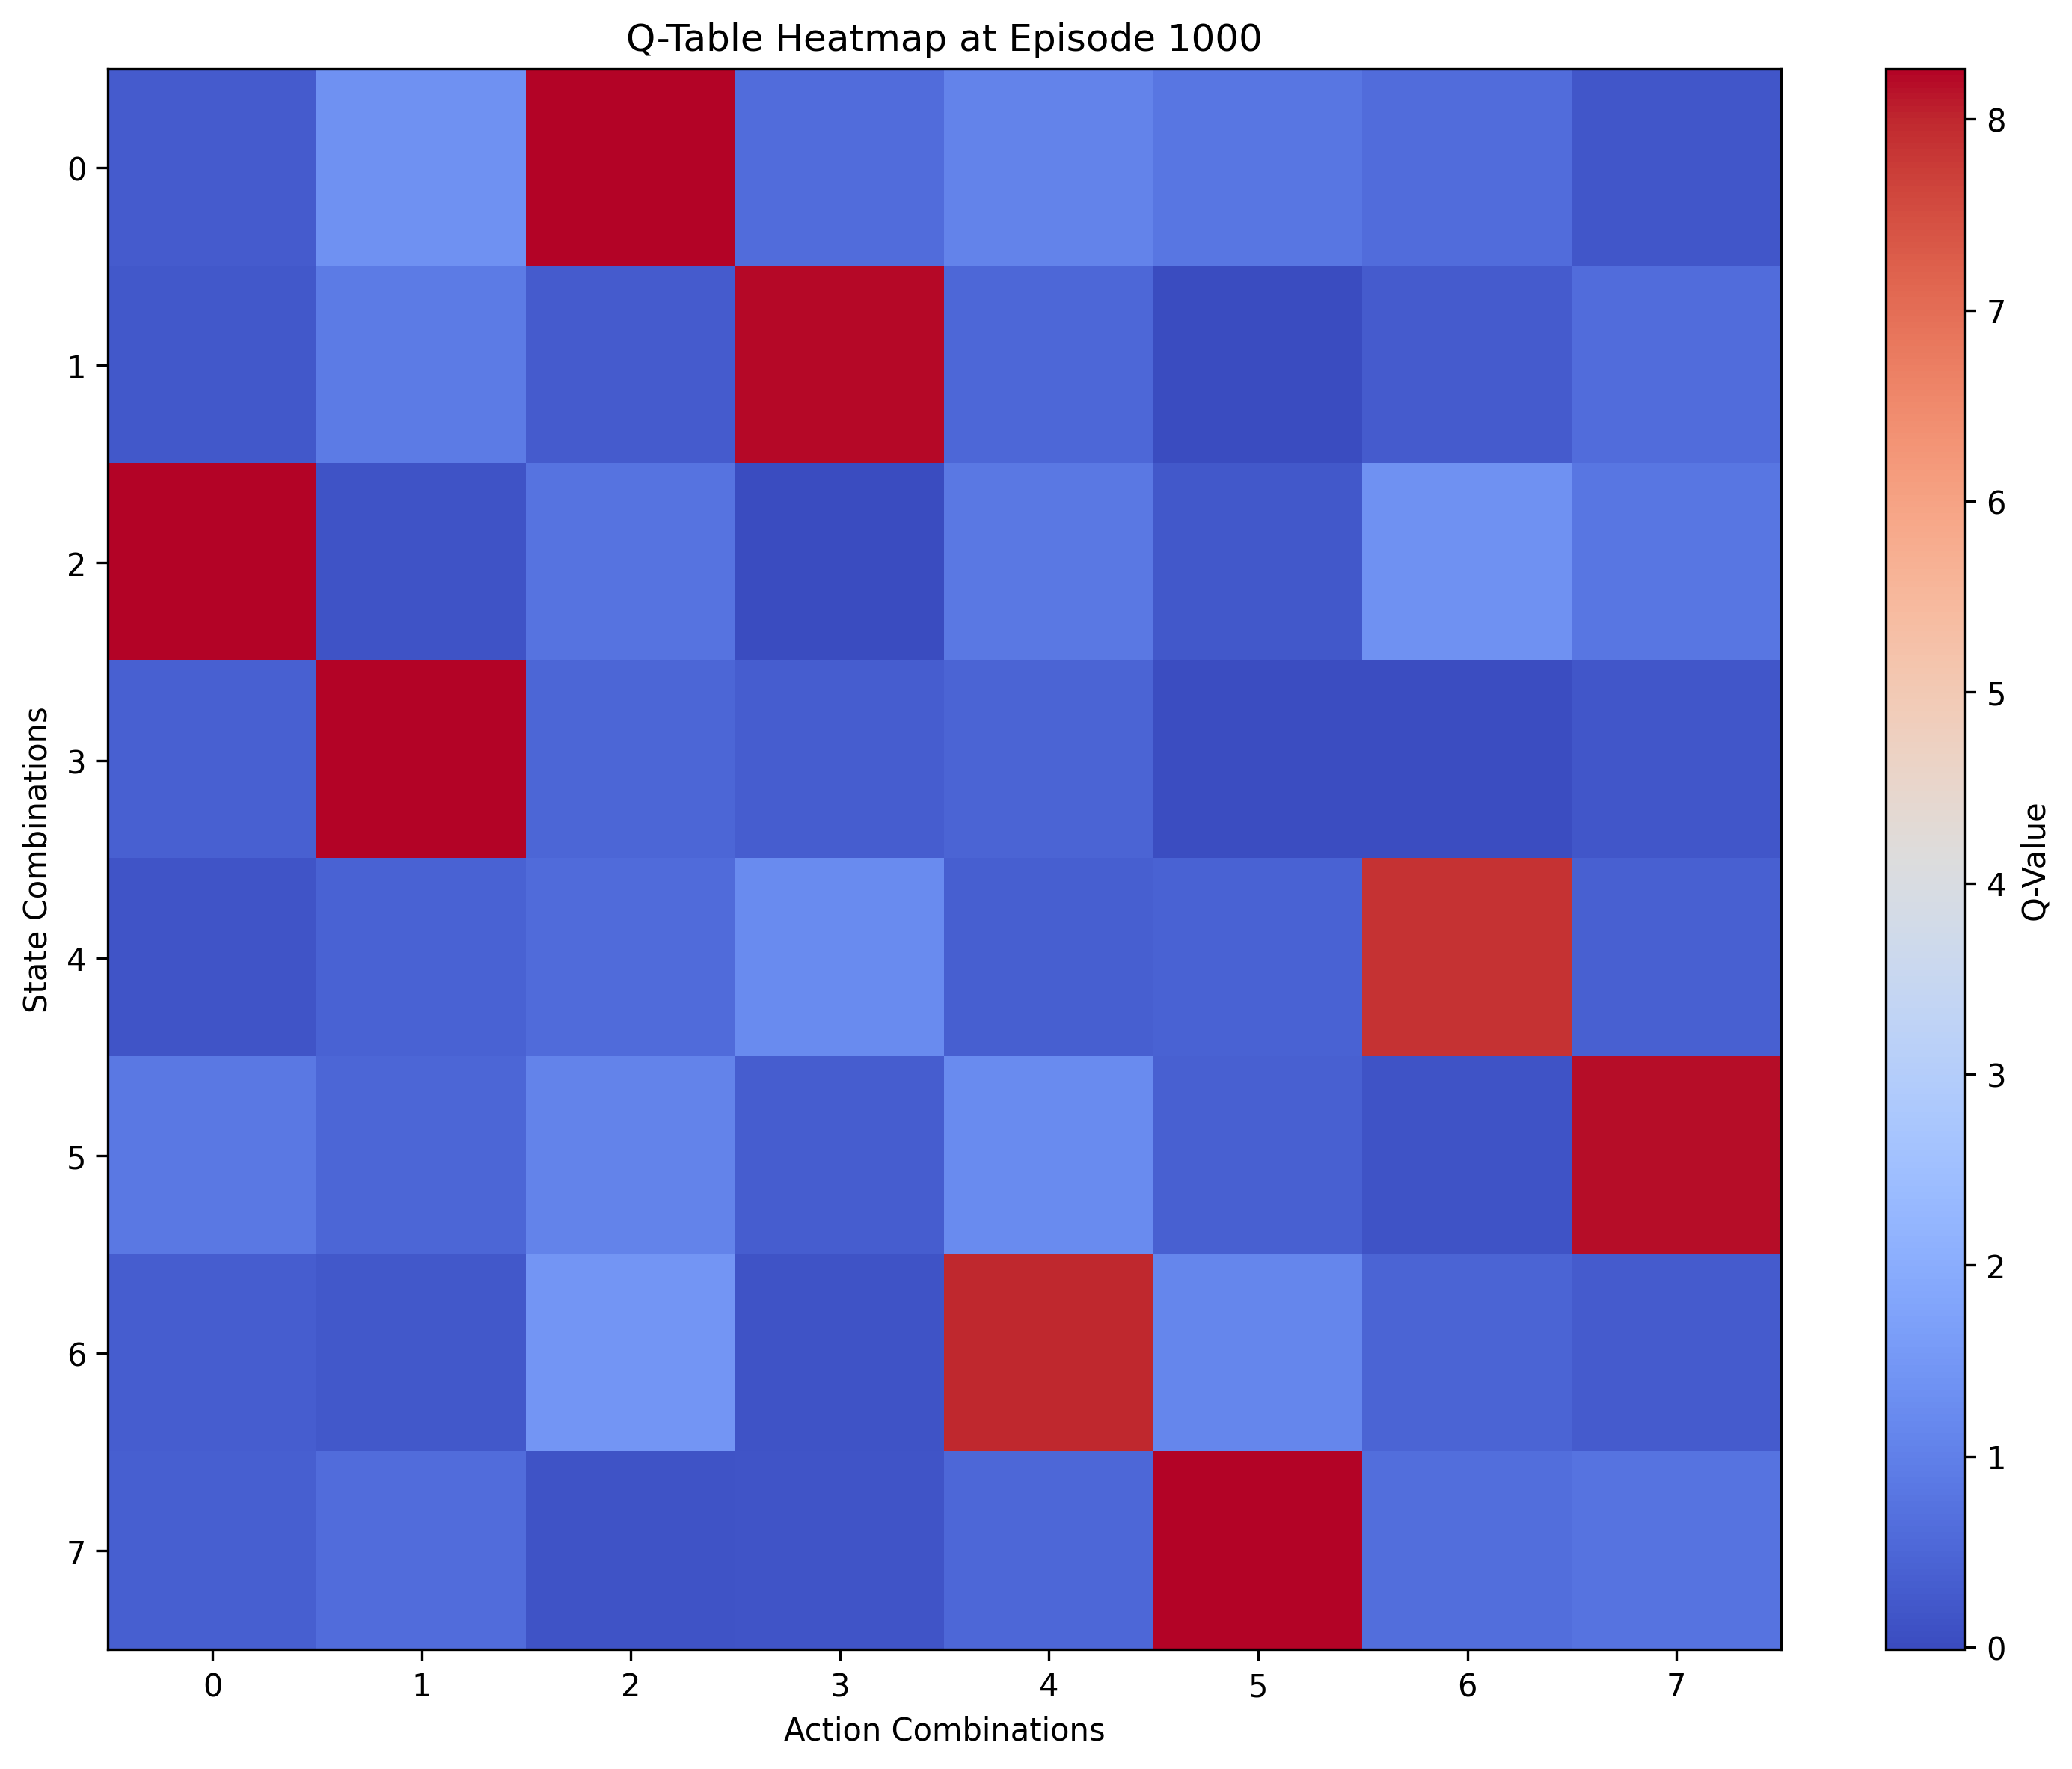
\includegraphics[width=\linewidth]{figure/multi_switch/q_heatmap_episode_1000.png}
        \centering (j) Episode 1000
    \end{minipage}

    \caption{训练过程中 \(Q\) 值热力图的演化(Episode 700–1000,每 100 回合)}
\end{figure}

最后,我们对于每一种章台的具体 \(Q\) 值分布(Top-\(3\))也进行了可视化,如图~\ref{fig:qvalue_top3} 所示。可以看到,随着训练的进行,智能体逐渐识别出哪些状态-动作对具有更高的回报,并将其 \(Q\) 值提升至更高水平。
注意,这里的动作是是否拨动开关的二进制表示(例如,\(000\) 表示不拨动任何开关,\(111\) 表示拨动所有开关)。
例如,对于目标状态 \(010\),我们现在处于 \(001\),最优动作是拨动第二和第三个开关(\(011\)),其对应的 \(Q\) 值大于 \(8.0\),表明这是一个高回报的动作选择。
\begin{figure}[htbp]
    \centering
    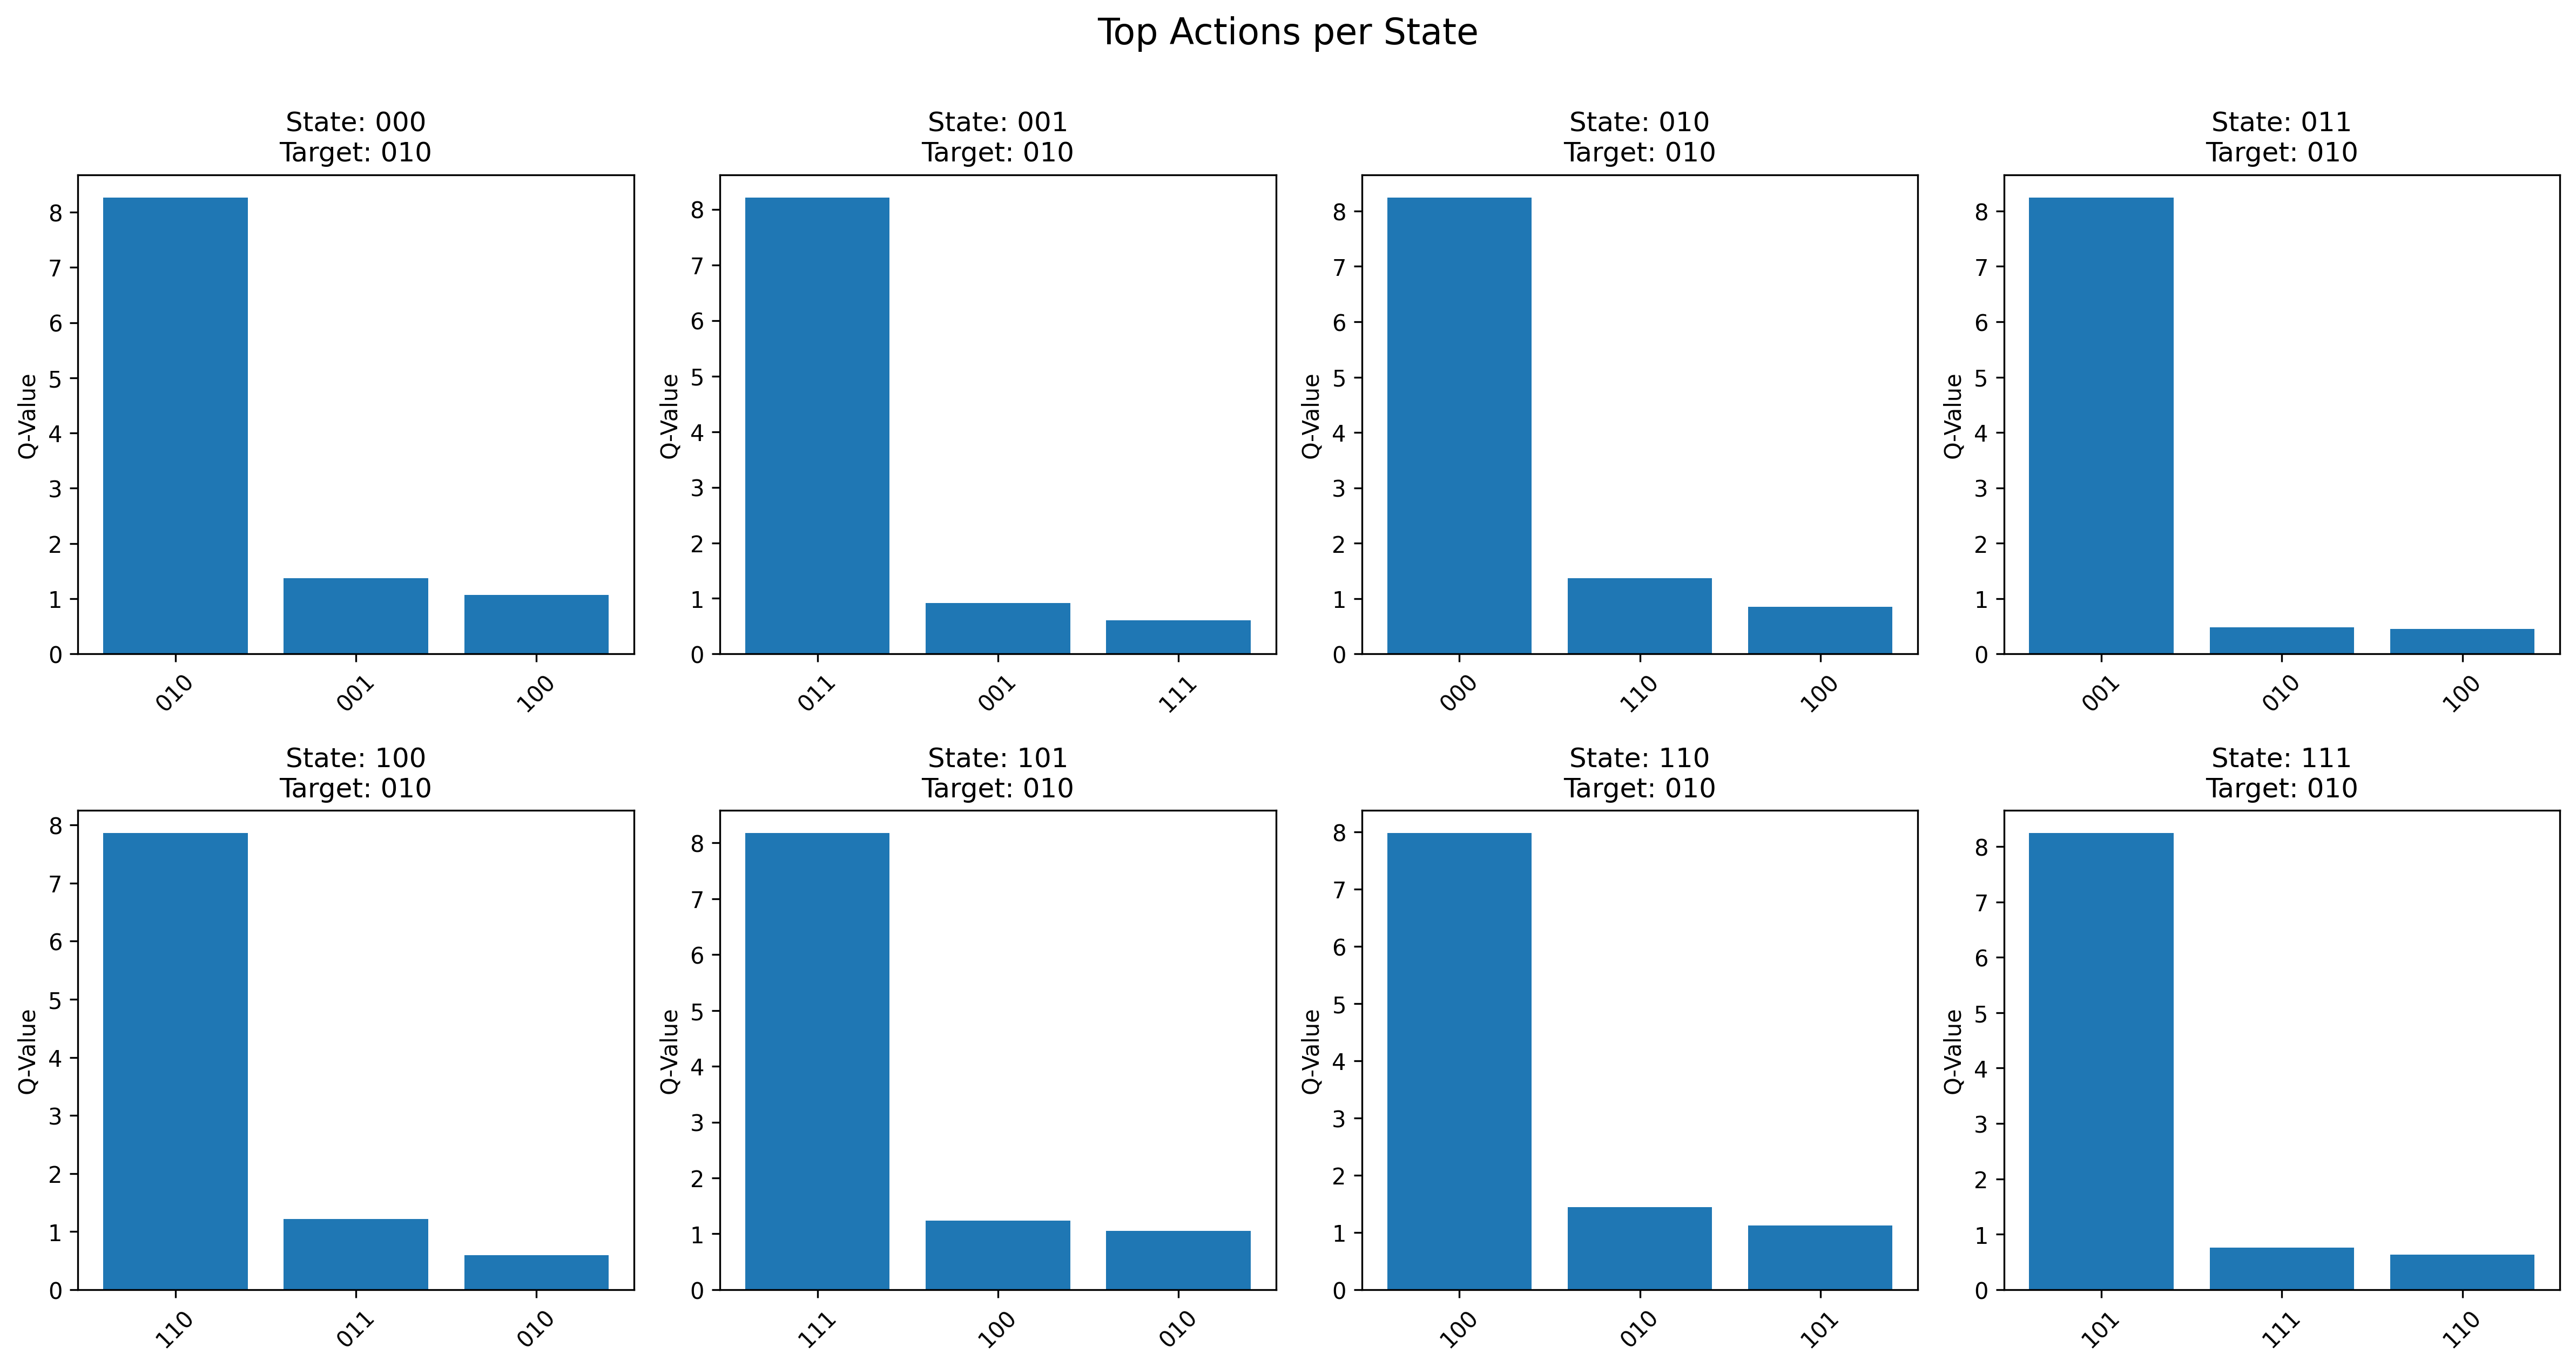
\includegraphics[width=1.0\textwidth]{figure/multi_switch/top_actions_visualization.png}
    \caption{每个状态下 \(Q\) 值最高的三个动作及其对应值(Top-\(3\))}
    \label{fig:qvalue_top3}
\end{figure}

\section{参数设置}

本实验的参数设置表~\ref{tab:multi-switch-params} 所示:

\begin{table}[htbp]
\centering
\caption{多开关环境Q-learning算法参数设置}
\label{tab:multi-switch-params}
\begin{tabular}{@{}lll@{}}
\toprule
\textbf{参数名称} & \textbf{含义} & \textbf{设置值} \\
\midrule
环境开关数量 (num\_switches) & 多开关环境中的开关数量 & 3 \\
状态空间维度 & 状态的二进制组合数量 & \( 2^3 = 8 \) \\
动作空间维度 & 动作的二进制组合数量 & \( 2^3 = 8 \) \\
\(Q\) 表维度 (\(Q\)-table shape) & 状态-动作组合的 Q 值表维度 & \( (2, 2, 2, 2, 2, 2) \) \\
学习率 \(\alpha\) & \(Q\)-learning 更新中步长系数 & 0.1 \\
折扣因子 \(\gamma\) & 未来奖励折扣权重 & 0.95 \\
初始探索率 (epsilon\_start) & \(\epsilon\)-贪婪策略初始探索概率 & 0.9 \\
最终探索率 (epsilon\_end) & \(\epsilon\)-贪婪策略最低探索概率 & 0.01 \\
探索率衰减 (epsilon\_decay) & 每轮训练后 \(\epsilon\) 的衰减倍数 & 0.995 \\
训练轮数 (episodes) & 总训练的回合数 & 1000 \\
测试轮数 (test\_episodes) & 测试阶段使用的轮数 & 10 \\
\bottomrule
\end{tabular}
\end{table}